\documentclass[xetex,mathserif,serif]{beamer}
\usepackage{polyglossia}
\setdefaultlanguage[babelshorthands=true]{russian}
\usepackage{minted}
\usepackage{tabu}
\usepackage{forest}
\usepackage[normalem]{ulem}

\usepackage{textpos}
\setlength{\TPHorizModule}{1cm}
\setlength{\TPVertModule}{1cm}

\usetikzlibrary{arrows}

\useoutertheme{infolines}

\setmainfont{FreeSans}
\newfontfamily{\russianfonttt}{FreeSans}

\definecolor{links}{HTML}{2A1B81}
\hypersetup{colorlinks,linkcolor=,urlcolor=links}

\tabulinesep=1.2mm

\newcommand{\attribution}[1] {
	\begin{flushright}\begin{scriptsize}\textcolor{gray}{\textcopyright\, #1}\end{scriptsize}\end{flushright}
}

\title{Продвинутые структуры данных}
\title{Хеш-таблицы, деревья}
\author[Юрий Литвинов]{Юрий Литвинов \newline \textcolor{gray}{\small\texttt{yurii.litvinov@gmail.com}}}
\date{06.04.2018г}

\begin{document}
	
	\frame{\titlepage}

	\section{Введение}

	\begin{frame}
		\frametitle{Абстрактные типы данных}
		\begin{itemize}
			\item АТД --- некоторая математическая модель и набор операций, определённый в рамках этой модели
			\begin{itemize}
				\item Обобщение понятия ``тип''
			\end{itemize}
			\item Состоит из типа данных и операций, выполняющих над ним преобразования
			\begin{itemize}
				\item Внутреннее устройство типа данных невидимо для остальной программы (принцип сокрытия деталей реализации)
				\item Работа с АТД --- только с помощью связанных с ним функций
				\item Тип данных и операции для работы с ним лежат рядом, так, чтобы все изменения в АТД были локализованы и не затрагивали остальную программу (принцип инкапсуляции)
			\end{itemize}
			\item В объектно-ориентированных языках АТД реализуется через классы
		\end{itemize}
	\end{frame}

	\begin{frame}
		\frametitle{Пример --- стек}
		\begin{itemize}
			\item Функции:
			\begin{itemize}
				\item createStack()
				\item deleteStack()
				\item push()
				\item pop()
				\item isEmpty()
			\end{itemize}
			\item \textbf{Внешнему миру вообще всё равно, как стек устроен внутри}
			\begin{itemize}
				\item Может быть на массиве
				\item Может быть на указателях
			\end{itemize}
		\end{itemize}
	\end{frame}

	\section{Деревья}

	\begin{frame}
		\frametitle{Дерево}
		\begin{columns}
			\begin{column}{0.6\textwidth}
				Ещё один абстрактный тип данных, используемый в программировании повсеместно
				\begin{itemize}
					\item Файловая система
					\item Абстрактное синтаксическое дерево
					\begin{itemize}
						\item Дерево разбора арифметического выражения
					\end{itemize}
					\item Двоичное дерево поиска
					\item Дерево контролов (или виджетов) в пользовательском интерфейсе
					\item ...
				\end{itemize}
			\end{column}
			\begin{column}{0.4\textwidth}
				\begin{center}
					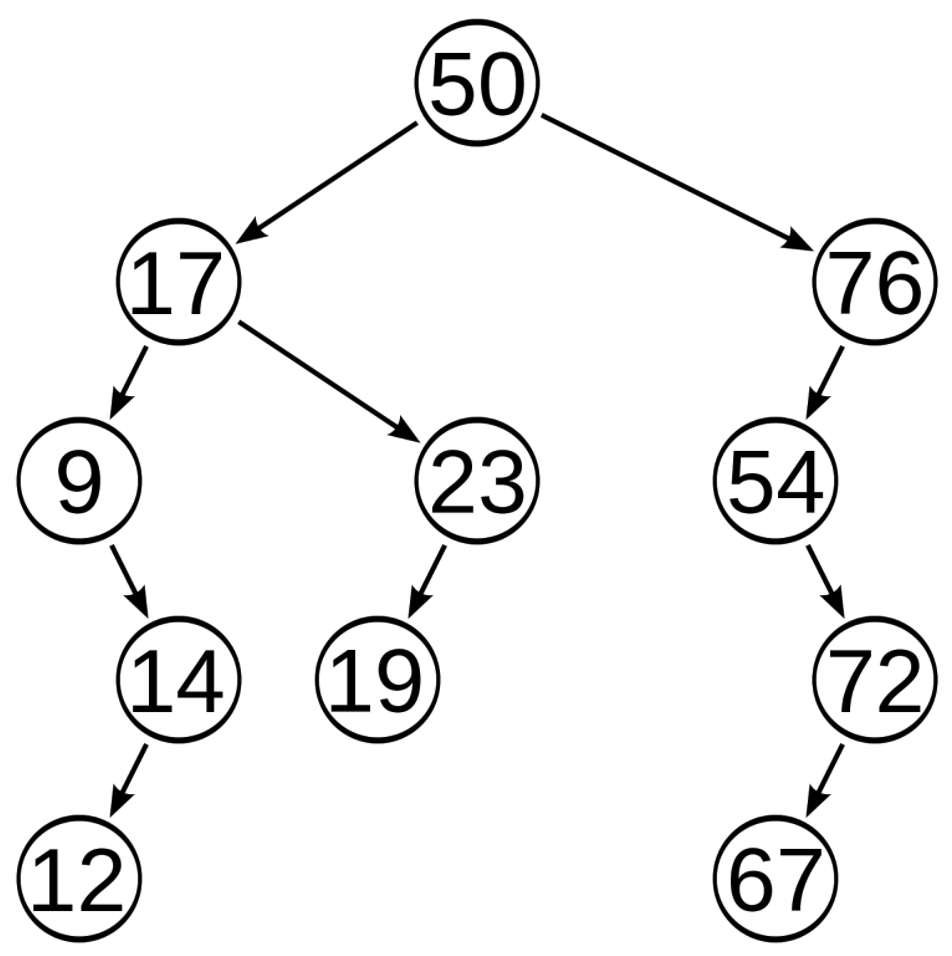
\includegraphics[width=0.9\textwidth]{tree.png}
				\end{center}
			\end{column}
		\end{columns}
	\end{frame}

	\begin{frame}
		\frametitle{Определения}
		Дерево --- совокупность элементов, называемых \textbf{узлами} (один из которых --- \textbf{корень}), и отношений, образующих иерархическую структуру узлов.
		\begin{itemize}
			\item Узел является деревом, он же --- корень дерева
			\item Есть узел $n$ и деревья $T_1$, $T_2$, ..., $T_k$ --- деревья с корнями $n_1$, $n_2$, ..., $n_k$ соответственно. Тогда можно построить новое дерево, с корнем $n$ и поддеревьями $T_1$, $T_2$, ..., $T_k$. Узлы $n_1$, $n_2$, ..., $n_k$ называются \textbf{сыновьями} узла $n$.
		\end{itemize}
		Нулевое дерево --- дерево без узлов.

		Дерево --- связный ациклический граф.

		Несвязный ациклический граф --- лес.
	\end{frame}

	\begin{frame}
		\frametitle{Ещё определения}
		\begin{itemize}
			\item Путь из $n_1$ в $n_k$ --- последовательность узлов $n_1$, ..., $n_k$, в которой каждый узел является родителем следующего
			\item Длина пути --- число, на единицу меньшее количества узлов, составляющих путь
			\item Путь нулевой длины --- путь из узла к самому себе
			\item Узел $a$ называется предком узла $b$, если существует путь из $a$ в $b$, $b$ в этом случае --- потомок $a$
			\begin{itemize}
				\item Каждый узел --- предок и потомок самого себя
			\end{itemize}
			\item Потомок, не являющийся самим узлом, называется истинным потомком
			\begin{itemize}
				\item C предком аналогично
			\end{itemize}
			\item Узел, не имеющий истинных потомков, называется листом
			\item Поддерево какого-либо дерева --- узел вместе со всеми потомками
		\end{itemize}
	\end{frame}

	\begin{frame}
		\frametitle{И ещё определения}
		\begin{itemize}
			\item Высота узла --- длина самого длинного пути из узла до какого-либо листа
			\item Глубина узла --- длина пути от узла до корня
			\item Высота дерева --- высота корня
			\item Деревья бывают упорядоченными и неупорядоченными
			\begin{itemize}
				\item Можно упорядочить узлы дерева, не связанные отношением предок-потомок (слева-справа)
			\end{itemize}
			\item Деревья бывают помеченными (каждой вершине сопоставлено значение)
		\end{itemize}
	\end{frame}

	\begin{frame}
		\frametitle{Обходы}
		В глубину:

		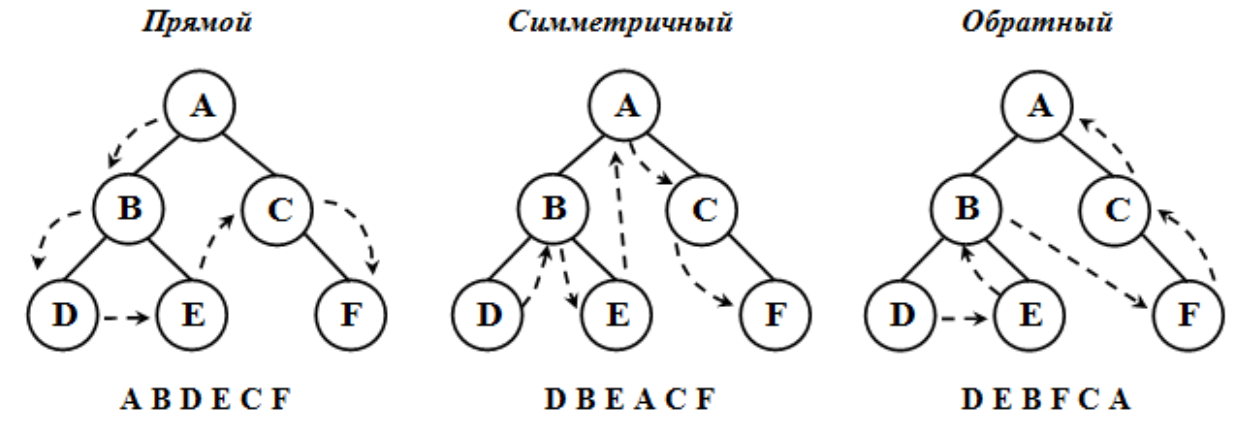
\includegraphics[width=0.6\textwidth]{treeDfs.png}

		\vspace{3mm}

		В ширину:

		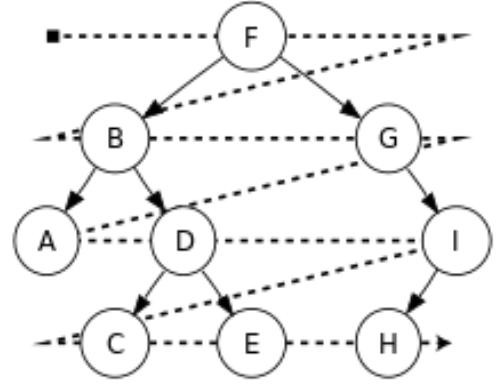
\includegraphics[width=0.25\textwidth]{treeBfs.png}
	\end{frame}

	\begin{frame}
		\frametitle{Деревья выражений}
		\begin{columns}
			\begin{column}{0.6\textwidth}
				$(a + b) * c + 7$
				\begin{itemize}
					\item Прямой порядок --- префиксная запись
					\begin{itemize}
						\item $+ * +\ a\ b\ c\ 7$
					\end{itemize}
					\item Обратный порядок --- постфиксная запись
					\begin{itemize}
						\item $a\ b + c * 7 +$
					\end{itemize}
					\item Симметричный порядок --- инфиксная запись
					\begin{itemize}
						\item $a + b * c + 7$
					\end{itemize}
				\end{itemize}
			\end{column}
			\begin{column}{0.4\textwidth}
				\begin{center}
					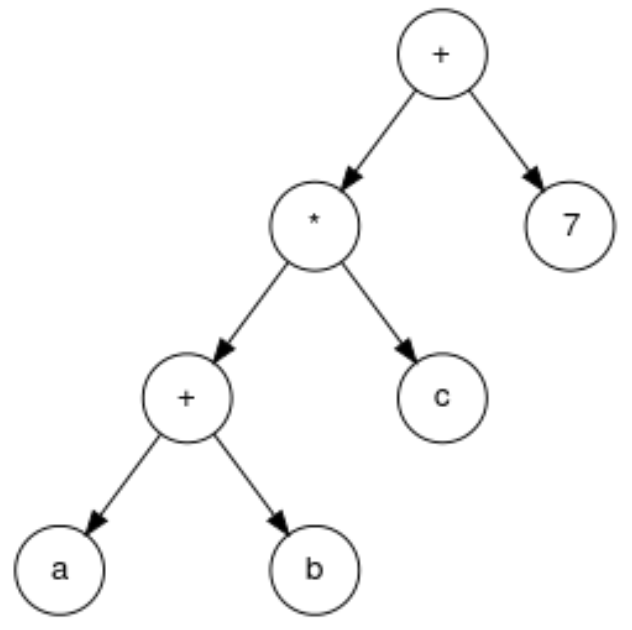
\includegraphics[width=0.9\textwidth]{expressionTree.png}
				\end{center}
			\end{column}
		\end{columns}
	\end{frame}

	\begin{frame}[fragile]
		\frametitle{АТД ``Дерево''}
		\begin{columns}
			\begin{column}{0.5\textwidth}
				\begin{itemize}
					\item parent(n, t)
					\item leftmostChild(n, t)
					\item rightSibling(n, t)
					\item label(n, t)
					\item create(n, t1, ..., ti)
					\item root(t)
					\item makenull(t)
				\end{itemize}
			\end{column}
			\begin{column}{0.5\textwidth}
				\begin{minted}{c++}
void preorder(Node *n)
{
    cout << label(n);
    Node *child = leftmostChild(n);
    while (child != nullptr)
    {
        preorder(child);
        child = rightSibling(child);
    }
}
				\end{minted}
			\end{column}
		\end{columns}
	\end{frame}

	\begin{frame}[fragile]
		\frametitle{Нерекурсивный обход в прямом порядке}
		\begin{small}
			\begin{minted}{c++}
void nonRecursivePreorder(Node *n) {
    stack<Node*> s;
    Node *current = n;
    while (true) {
        if (current != nullptr) {
            cout << label(current) << " ";
            s.push(current);
            current = leftmostChild(current);
        } else {
            if (s.empty())
                return;
            current = rightSibling(s.top());
            s.pop();
        }
    }
}
			\end{minted}
		\end{small}
	\end{frame}

	\begin{frame}[fragile]
		\frametitle{Реализация списком сыновей}
		\begin{columns}
			\begin{column}{0.4\textwidth}
				\begin{minted}{c++}
struct Node
{
    ElementType value;
    Node *sibling;
    Node *child;
};
				\end{minted}
			\end{column}
			\begin{column}{0.6\textwidth}
				\begin{center}
					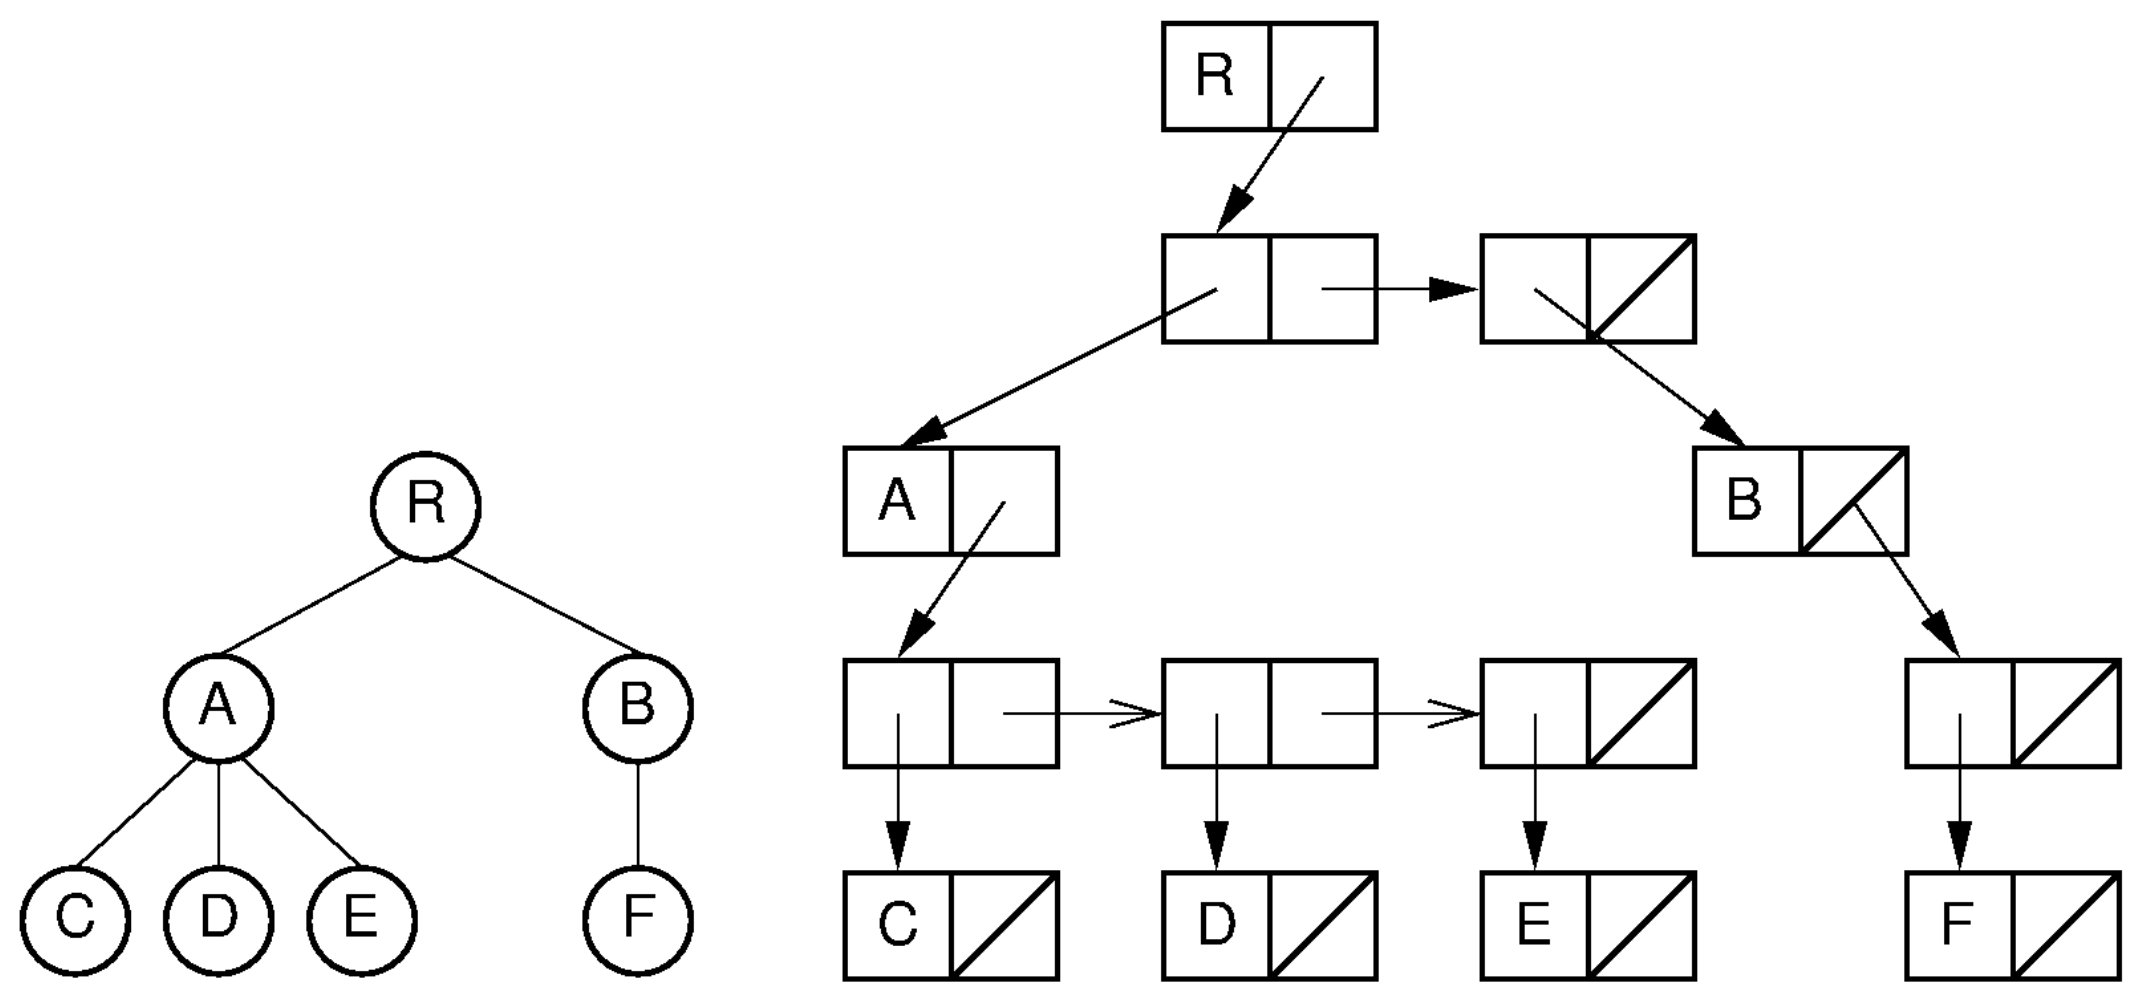
\includegraphics[width=\textwidth]{childListTree.png}
				\end{center}
			\end{column}
		\end{columns}
	\end{frame}

	\begin{frame}[fragile]
		\frametitle{Двоичные деревья}
		Деревья, у которых есть левый и правый сын, и это разные вещи
		\begin{columns}
			\begin{column}{0.5\textwidth}
				\begin{minted}{c++}
struct Node
{
    ElementType value;
    Node *leftChild;
    Node *rightChild;
};
				\end{minted}
			\end{column}
			\begin{column}{0.5\textwidth}
				\begin{center}
					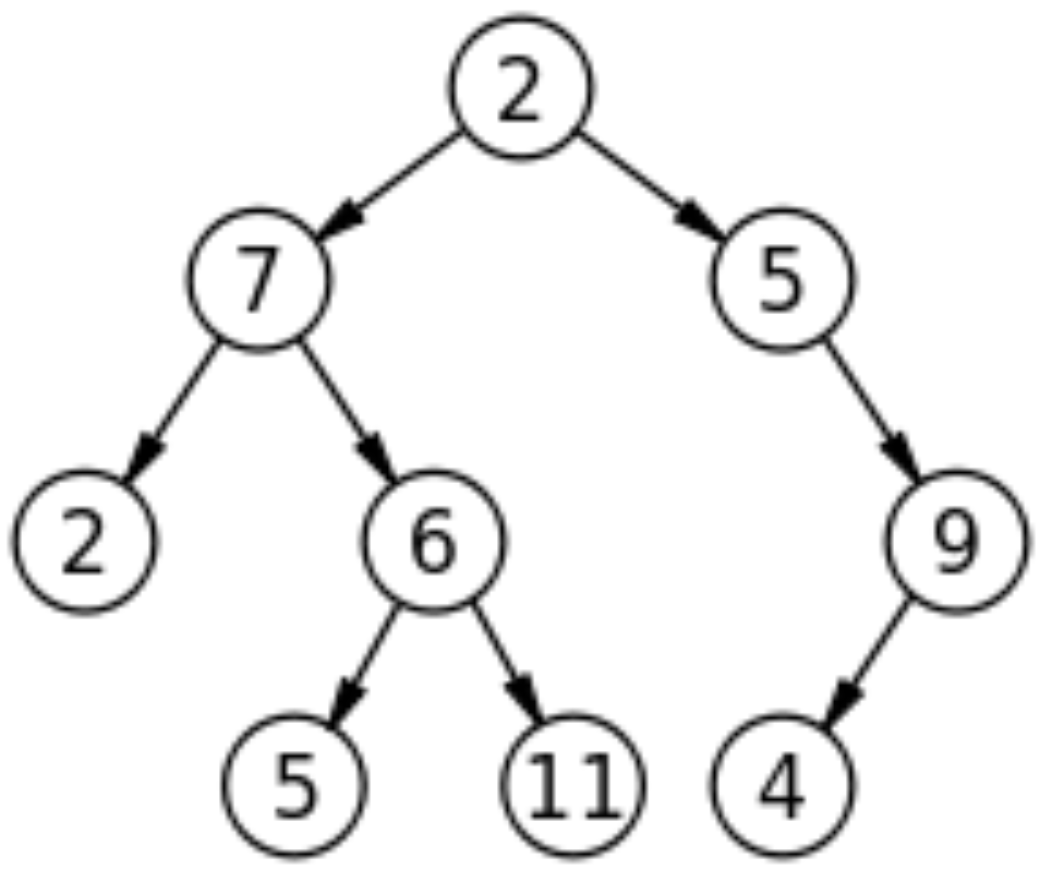
\includegraphics[width=0.6\textwidth]{binaryTree.png}
				\end{center}
			\end{column}
		\end{columns}
	\end{frame}

	\begin{frame}
		\frametitle{Пример: алгоритм Хаффмана}
		\begin{columns}
			\begin{column}{0.4\textwidth}
				\begin{itemize}
					\item Алгоритм сжатия, вычисляющий кратчайшую кодовую последовательность для символа
					\begin{itemize}
						\item Если в тексте одни буквы ``А'', нет смысла кодировать А 16-ю битами
					\end{itemize}
					\item Префиксные коды
					\item Дерево частот символов
				\end{itemize}
			\end{column}
			\begin{column}{0.6\textwidth}
				\begin{center}
					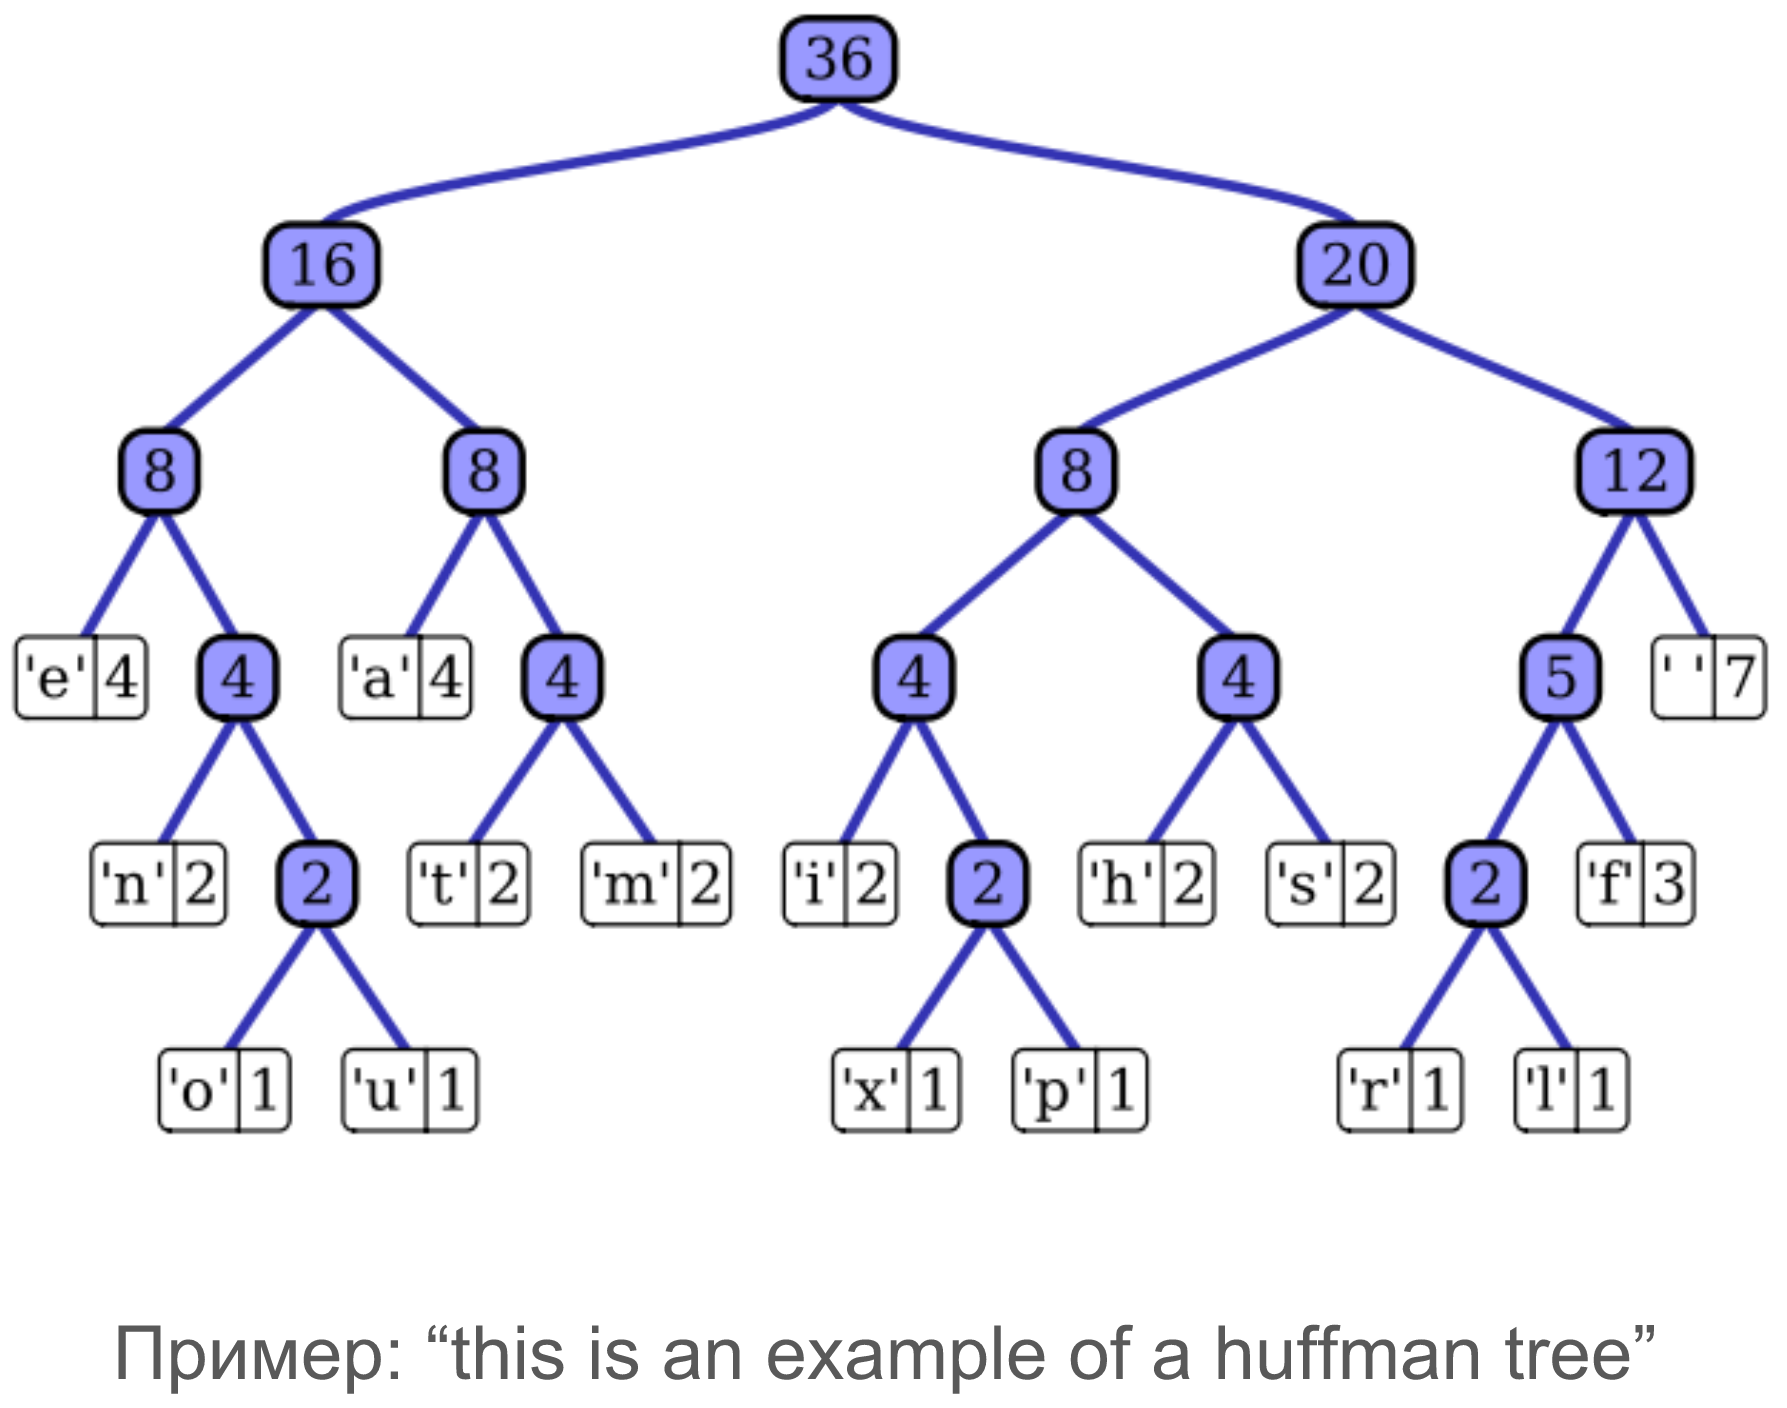
\includegraphics[width=0.9\textwidth]{huffmanTree.png}
				\end{center}
			\end{column}
		\end{columns}
	\end{frame}

	\begin{frame}
		\frametitle{Двоичное дерево поиска}
		\begin{columns}
			\begin{column}{0.6\textwidth}
				\begin{itemize}
					\item Двоичное дерево, у которого для каждого узла в левом поддереве элементы, меньшие значения в узле, в правом --- элементы, большие значения в узле
					\item Используется для представления множеств и ассоциативных массивов
					\begin{itemize}
						\item Если дерево сбалансировано (т.е. высота примерно логарифм количества вершин), операции вставки, удаления и поиска выполняются за log(n)
					\end{itemize}
				\end{itemize}
			\end{column}
			\begin{column}{0.4\textwidth}
				\begin{center}
					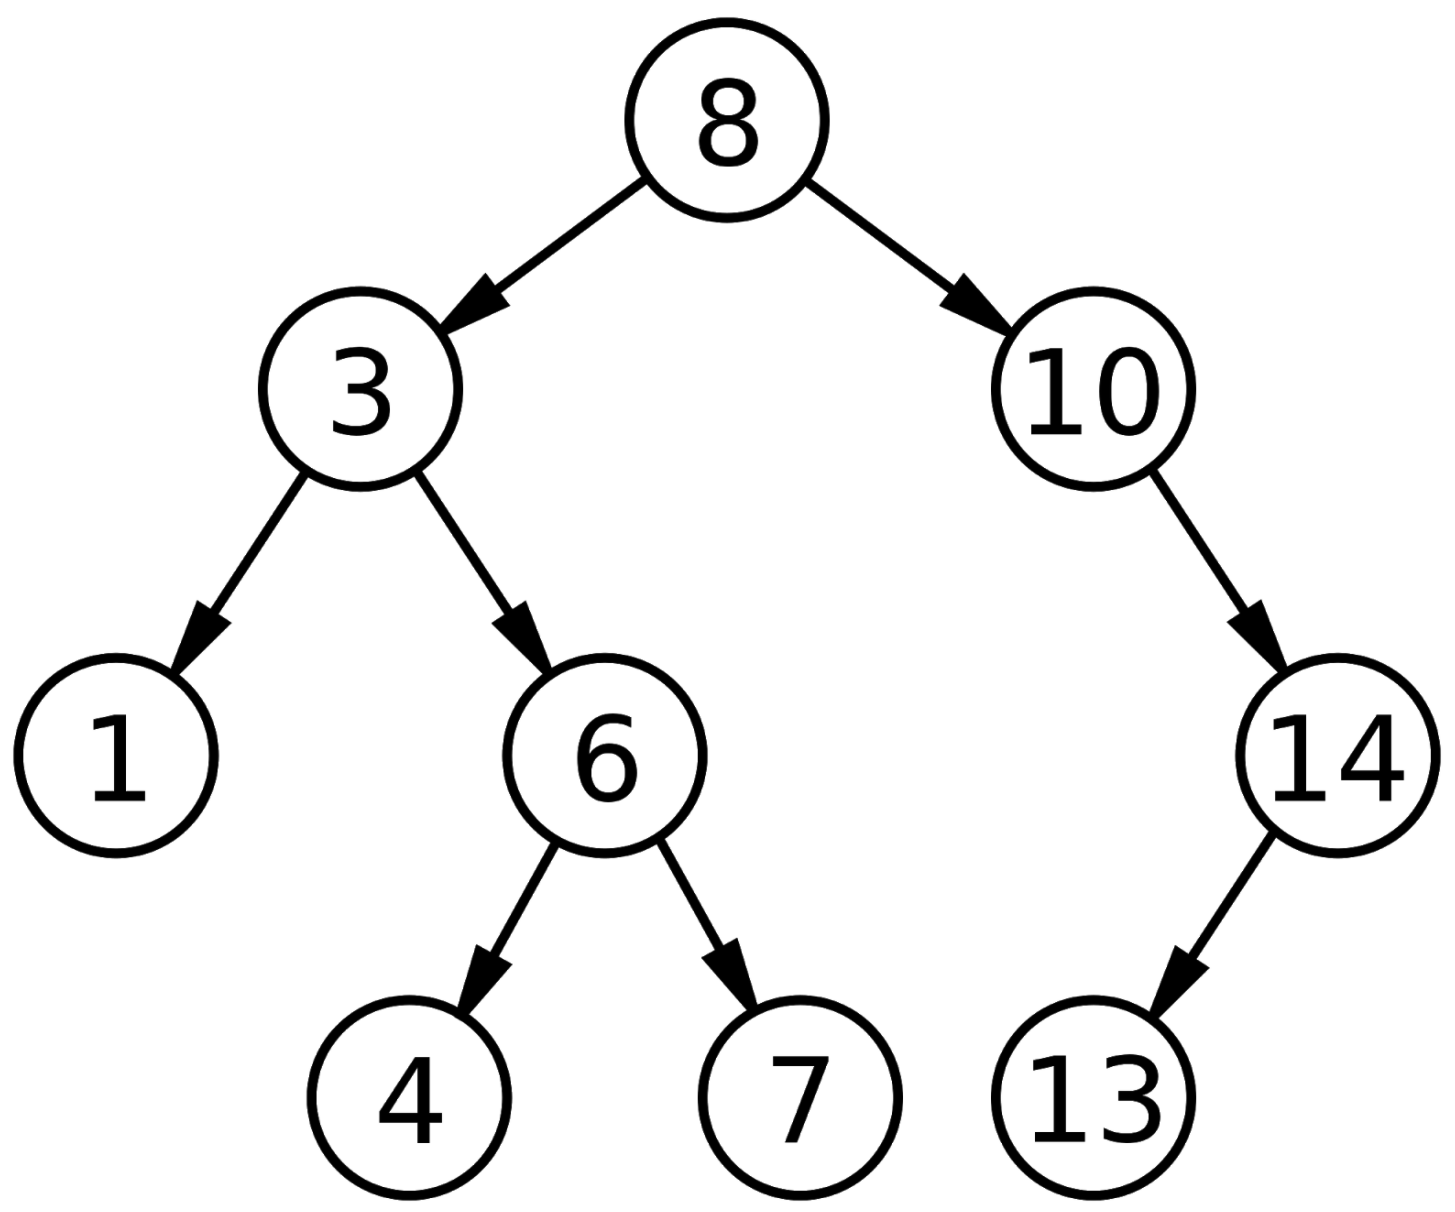
\includegraphics[width=0.9\textwidth]{bst.png}
				\end{center}
			\end{column}
		\end{columns}
	\end{frame}

	\begin{frame}
		\frametitle{Операции}
		\begin{columns}
			\begin{column}{0.5\textwidth}
				Вставка:

				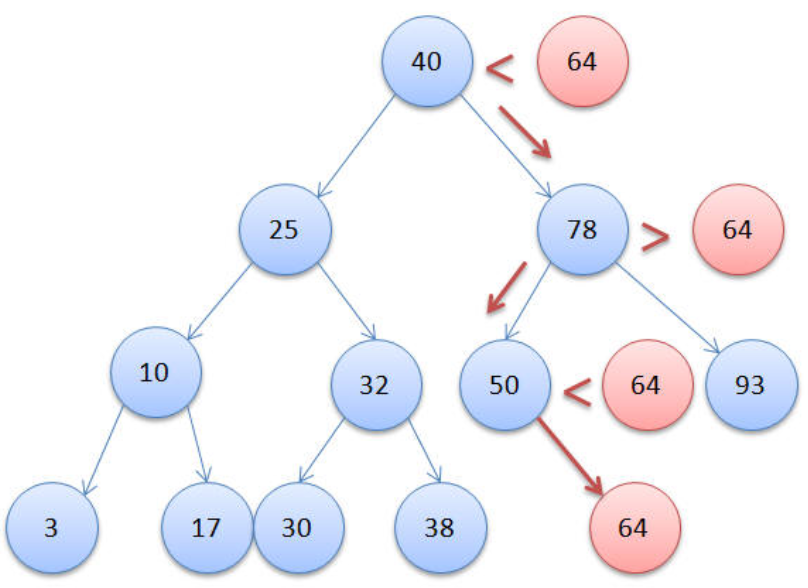
\includegraphics[width=0.9\textwidth]{bstInsertion.png}
			\end{column}
			\begin{column}{0.5\textwidth}
				Удаление:

				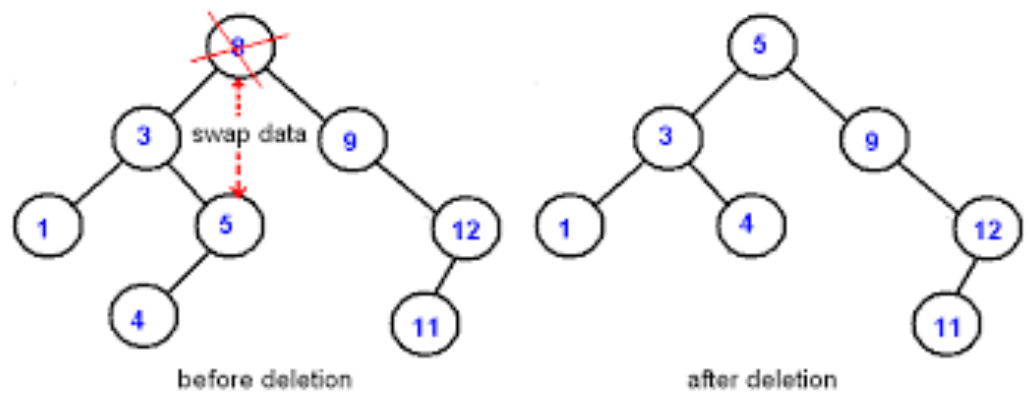
\includegraphics[width=0.9\textwidth]{bstRemoval.png}
			\end{column}
		\end{columns}
	\end{frame}

	\begin{frame}
		\frametitle{Проблема}
		\begin{columns}
			\begin{column}{0.4\textwidth}
				\begin{itemize}
					\item При неудачном порядке вставки дерево может выродиться в список
					\item $n <= 2^{h + 1} - 1$, поэтому $h >= log_2(n + 1) - 1 >= floor(log_2(n))$
					\item Трудоёмкости всех операций сразу станут линейными
				\end{itemize}
			\end{column}
			\begin{column}{0.6\textwidth}
				\begin{center}
					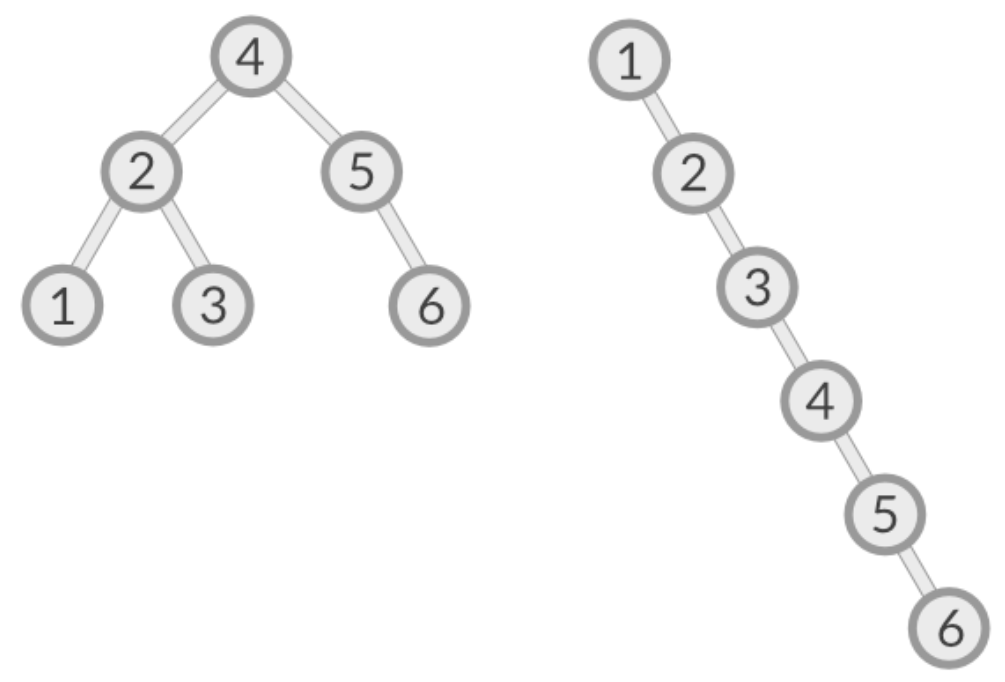
\includegraphics[width=0.9\textwidth]{badBst.png}
				\end{center}
			\end{column}
		\end{columns}
	\end{frame}

	\section{Самобалансирующиеся деревья}

	\begin{frame}
		\frametitle{Балансировка}
		\begin{columns}
			\begin{column}{0.6\textwidth}
				\begin{itemize}
					\item Перестраиваем дерево каждый раз после вставки и удаления, чтобы сохранить высоту дерева возможно меньшей
					\item Основная операция --- поворот
					\begin{itemize}
						\item Сохраняет свойства двоичного дерева поиска
						\item Возможно, уменьшает его общую высоту
					\end{itemize}
					\item Конкретных алгоритмов балансировки очень много
				\end{itemize}
			\end{column}
			\begin{column}{0.4\textwidth}
				\begin{center}
					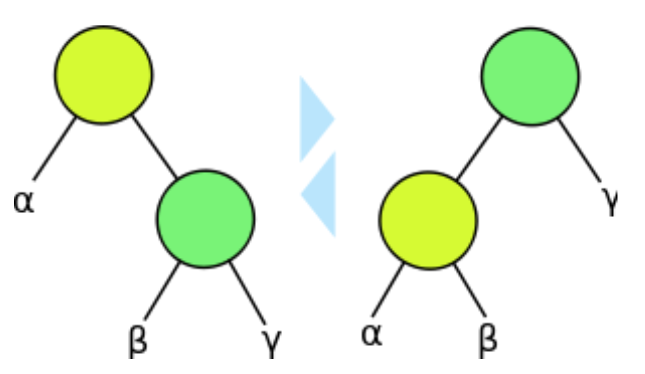
\includegraphics[width=\textwidth]{rotation.png}
				\end{center}
			\end{column}
		\end{columns}
	\end{frame}

	\begin{frame}
		\frametitle{АВЛ-дерево}
		\begin{columns}
			\begin{column}{0.6\textwidth}
				\begin{itemize}
					\item 1962г., Г.М. Адельсон-Вельский и Е.М. Ландис
					\item В каждой вершине хранится разность высот левого и правого поддерева
					\item Вставка и удаление гарантируют, что разность высот будет не больше 1
					\item Теоретически лучшая балансировка из популярных деревьев, но относительно большой оверхэд
				\end{itemize}
			\end{column}
			\begin{column}{0.4\textwidth}
				\begin{center}
					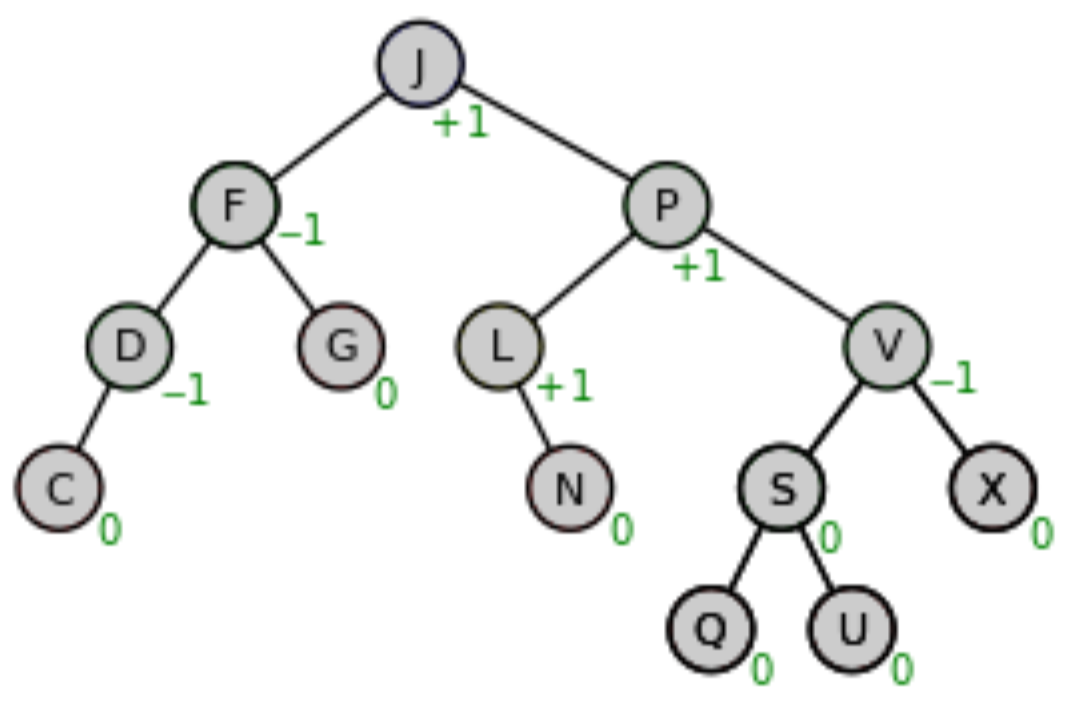
\includegraphics[width=\textwidth]{avlTree.png}
				\end{center}
			\end{column}
		\end{columns}
	\end{frame}

	\begin{frame}
		\frametitle{Балансировка}
		\begin{columns}
			\begin{column}{0.5\textwidth}
				Малое левое вращение

				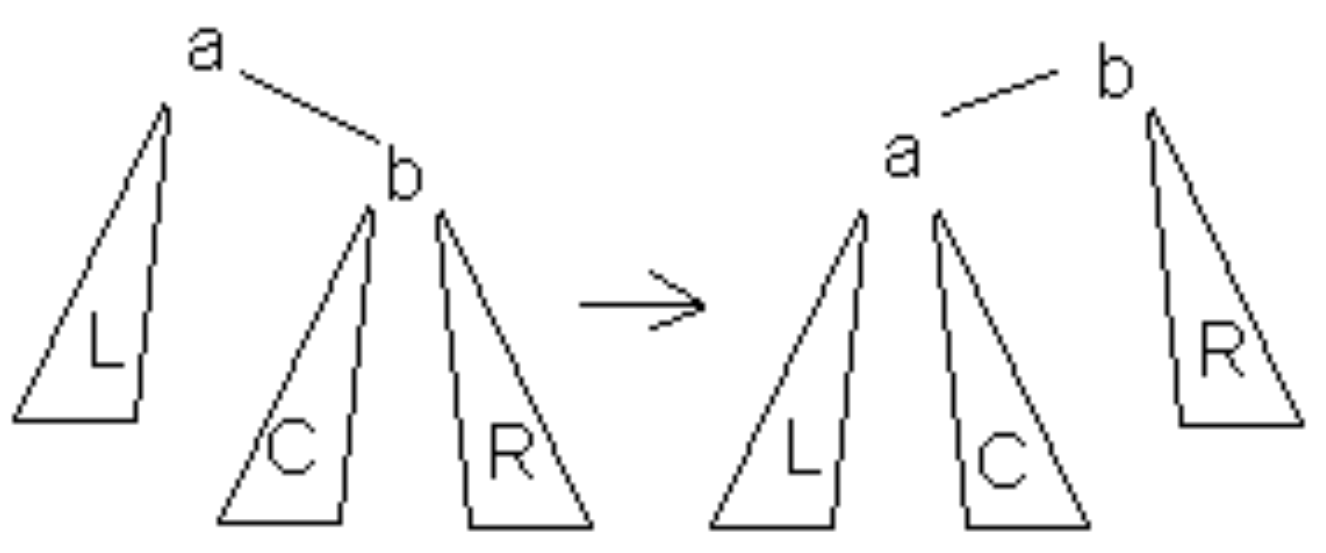
\includegraphics[width=0.8\textwidth]{avlSmallLeft.png}
			\end{column}
			\begin{column}{0.5\textwidth}
				Малое правое вращение

				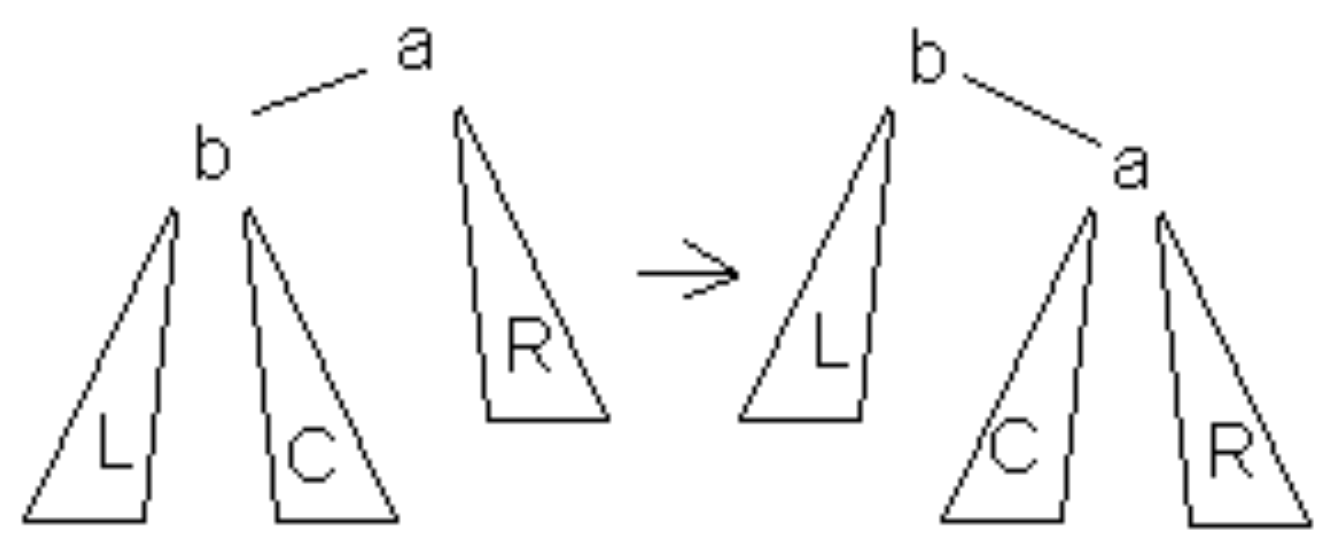
\includegraphics[width=0.8\textwidth]{avlSmallRight.png}
			\end{column}
		\end{columns}
		\vspace{3mm}
		Проводится в случае, если высота b > высота L + 1, и высота C <= высоте R
		\begin{itemize}
			\item При повороте важно не забыть обновить значения баланса
			\item И не запутаться в указателях
		\end{itemize}
	\end{frame}

	\begin{frame}
		\frametitle{Балансировка}
		\begin{columns}
			\begin{column}{0.5\textwidth}
				Большое левое вращение

				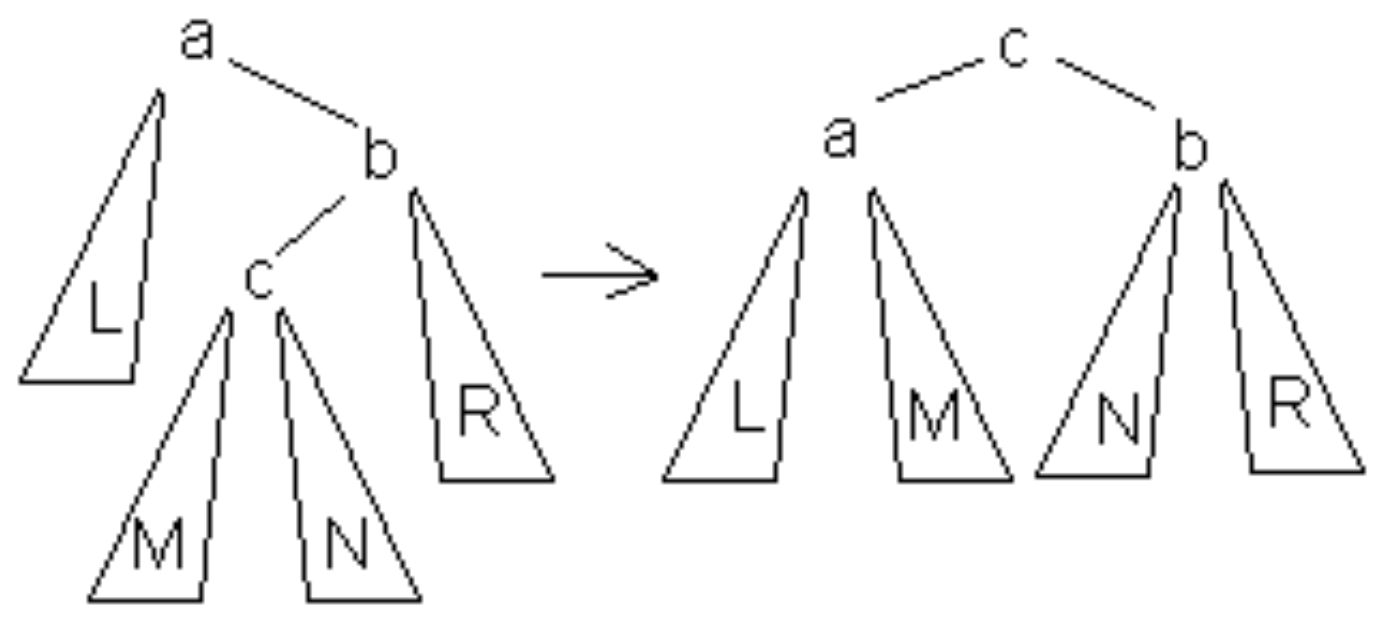
\includegraphics[width=0.8\textwidth]{avlLargeLeft.png}
			\end{column}
			\begin{column}{0.5\textwidth}
				Большое правое вращение

				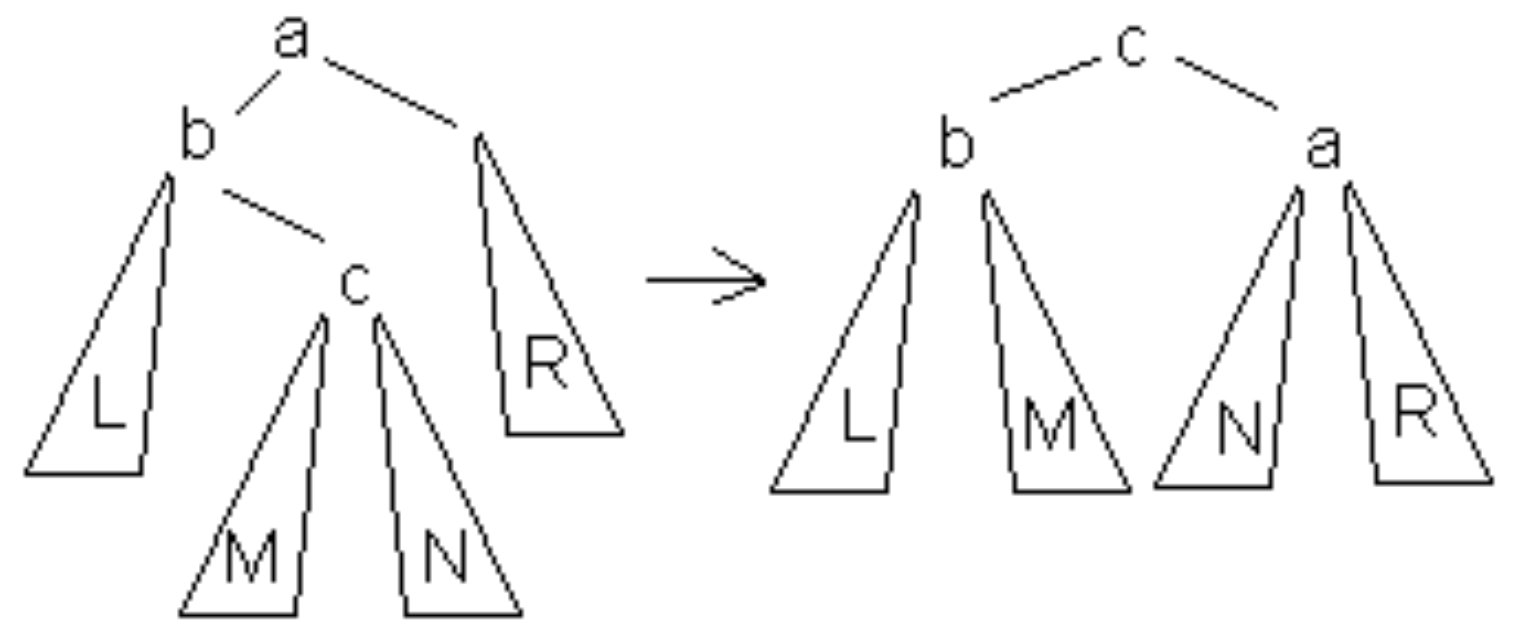
\includegraphics[width=0.8\textwidth]{avlLargeRight.png}
			\end{column}
		\end{columns}
		\vspace{3mm}
		Балансировка выполняется на обратном проходе рекурсии при вставке и удалении, если есть потребность
	\end{frame}

	\begin{frame}
		\frametitle{Красно-чёрные деревья}
		\begin{itemize}
			\item 1972г., Р. Байер
			\item Хуже сбалансированы, чем АВЛ-деревья, зато \sout{не придуманы в Советском Союзе} требуют константного количества поворотов на каждую операцию (в отличие от O(log(n)) для АВЛ-деревьев)
			\begin{itemize}
				\item Поэтому используются практически во всех стандартных библиотеках
			\end{itemize}
		\end{itemize}
	\end{frame}

	\begin{frame}
		\frametitle{Красно-чёрные деревья}
		\begin{itemize}
			\item В каждой вершине хранится цвет (красный или чёрный)
			\begin{itemize}
				\item Корень чёрный
				\item Все листья чёрные
				\item Оба потомка красного узла --- чёрные
				\item Всякий путь от данного узла до любого листового узла, являющегося его потомком, содержит одинаковое число чёрных узлов
				\begin{itemize}
					\item Высота поддеревьев не может отличаться более, чем вдвое
				\end{itemize}
			\end{itemize}
		\end{itemize}
		\begin{center}
			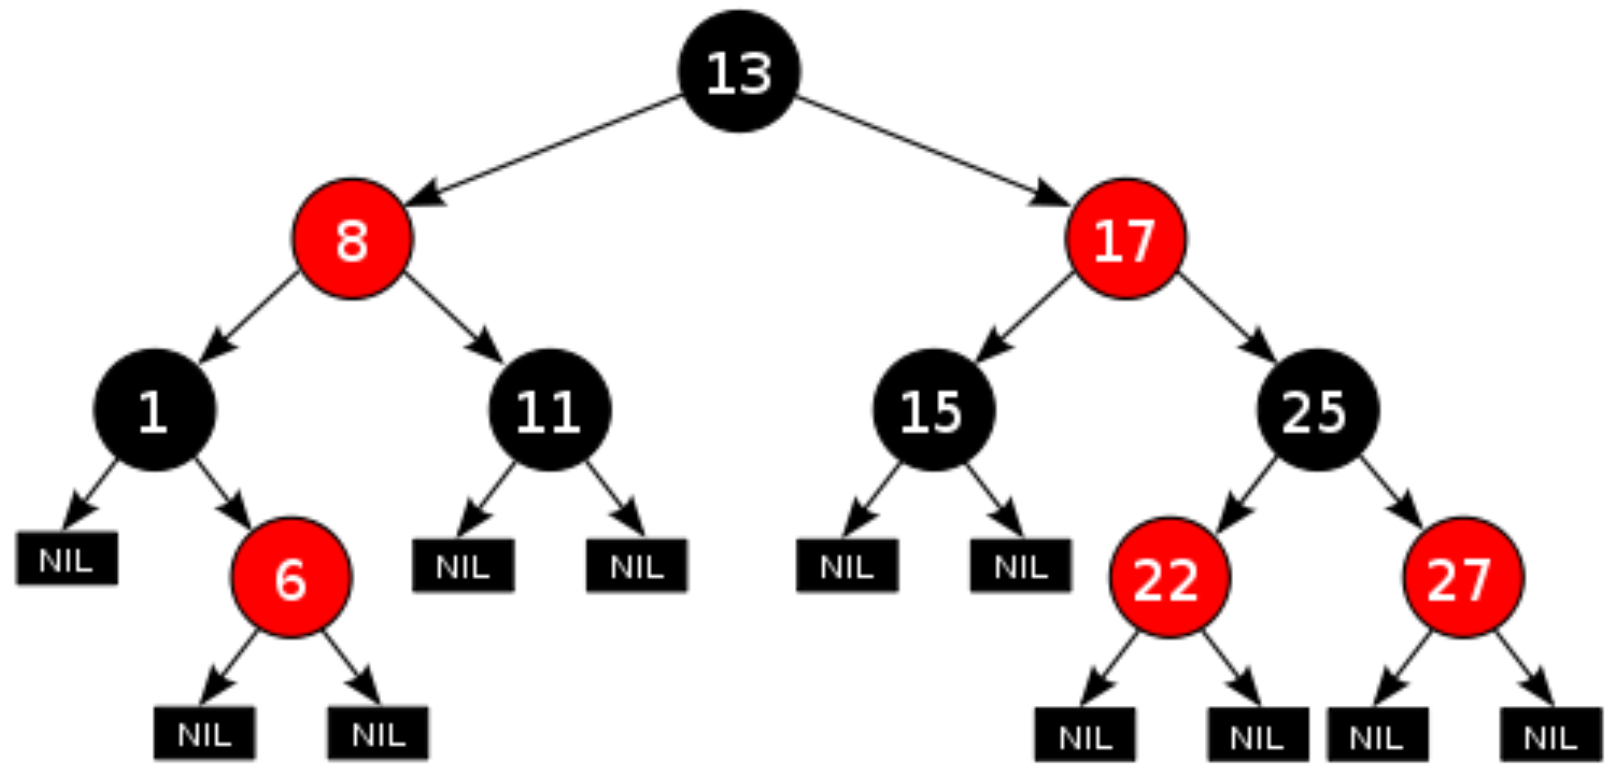
\includegraphics[width=0.5\textwidth]{redBlackTree.png}
		\end{center}
	\end{frame}

	\begin{frame}
		\frametitle{Красно-чёрное дерево, добавление}
		\framesubtitle{Случаи 1-3}
		\begin{columns}
			\begin{column}{0.5\textwidth}
				\begin{itemize}
					\item Добавляем в корень --- ок, красим его в чёрный
					\item Добавляем как сына чёрному узлу --- ок, красим в красный
					\item Если родитель и ``дядя'' красные, перекрашиваем их и добавляем наш узел как красный. Дедушка может нарушить ограничения, так что, возможно, его тоже придётся перекрасить (выполнив перекрашивание рекурсивно до корня)
				\end{itemize}
			\end{column}
			\begin{column}{0.5\textwidth}
				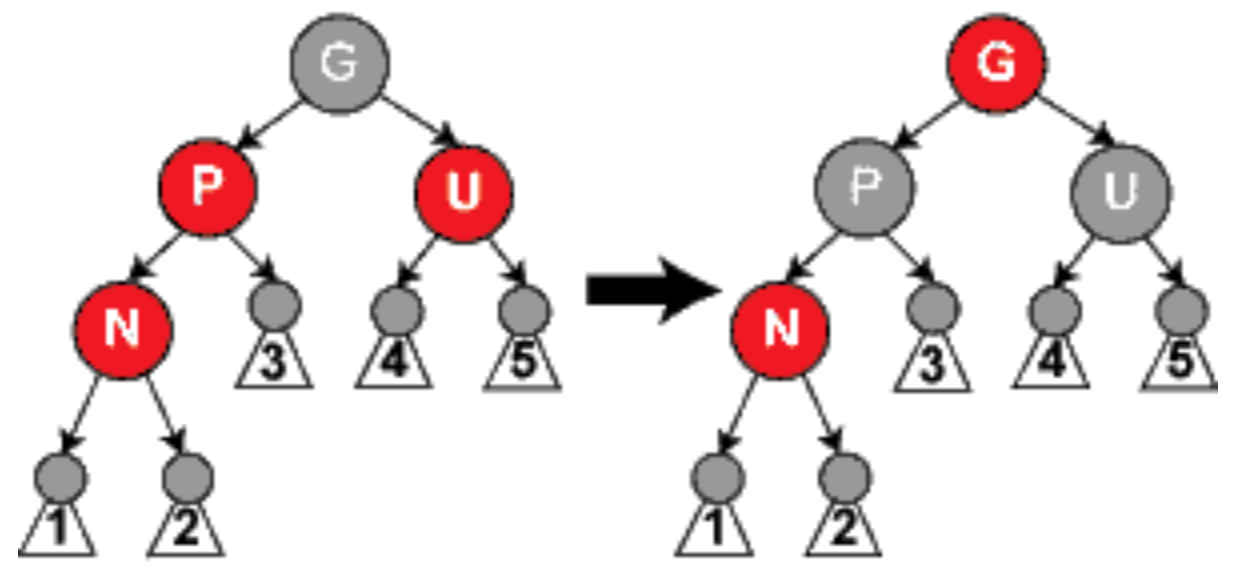
\includegraphics[width=0.8\textwidth]{redBlackAdding1.png}
			\end{column}
		\end{columns}
	\end{frame}

	\begin{frame}
		\frametitle{Красно-чёрное дерево, добавление}
		\framesubtitle{Случай 4}
		\begin{itemize}
			\item Родитель красный, дядя чёрный, узел справа от родителя. Выполняем поворот пары ``родитель-сын''.
			\begin{center}
				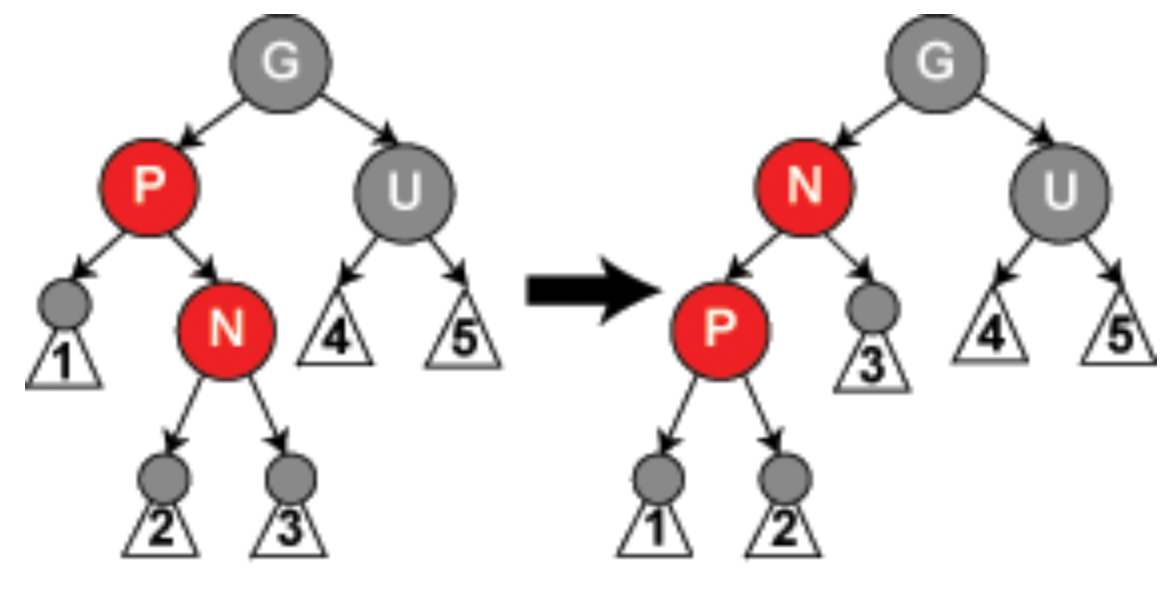
\includegraphics[width=0.4\textwidth]{redBlackAdding2.png}
			\end{center}
		\end{itemize}
		Ограничение ``оба потомка красного узла чёрные'' всё ещё нарушается, но об этом позаботится случай 5.
	\end{frame}

	\begin{frame}
		\frametitle{Красно-чёрное дерево, добавление}
		\framesubtitle{Случай 5}
		\begin{itemize}
			\item Родитель красный, дядя чёрный, узел слева от родителя. Выполняем поворот относительно пары ``родитель-дедушка'', который и восстанавливает балансировку.
			\begin{center}
				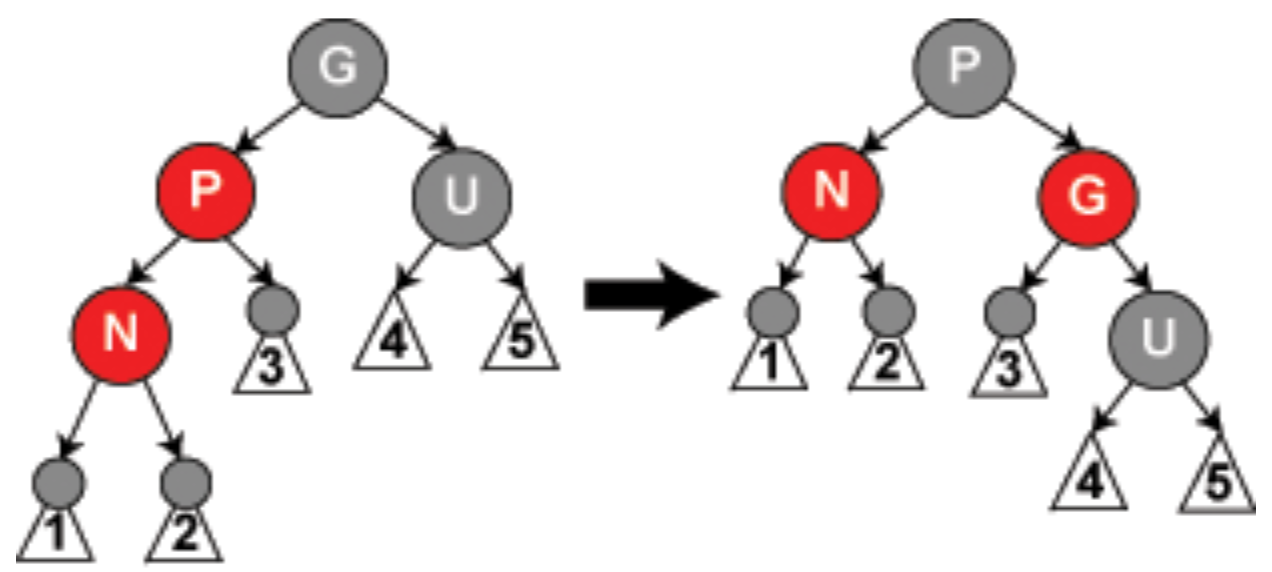
\includegraphics[width=0.4\textwidth]{redBlackAdding3.png}
			\end{center}
		\end{itemize}
		Опять-таки, надо не забыть перекрасить узлы
	\end{frame}

	\begin{frame}
		\frametitle{Красно-чёрное дерево, удаление}
		Сначала делаем как обычно --- кладём значение самого большого узла в левом поддереве в удаляемый узел и... надо удалить тот узел, откуда мы взяли значение, но не всё так просто.
		\begin{itemize}
			\item Если он красный, то оба его потомка --- чёрные листы. Удаляем красный узел и ставим на его место лист (они не хранят значений, поэтому не важно, какой)
			\item Если он чёрный, а его единственный нелистовой потомок красный, то ставим потомка на его место и перекрашиваем его в чёрный
			\item Если он чёрный и его потомок чёрный, то его оба потомка листы, но если кого-то просто удалить, то число чёрных узлов в поддереве изменится, так что надо перебалансировать дерево
		\end{itemize}
	\end{frame}

	\begin{frame}
		\frametitle{Красно-чёрное дерево, удаление}
		\framesubtitle{Случаи 1-2}
		\begin{itemize}
			\item Самый простой случай, когда удаляемый узел корень: просто удаляем
			\item У удалённого узла был красный брат: делаем поворот по ребру ``отец-брат''
			\begin{center}
				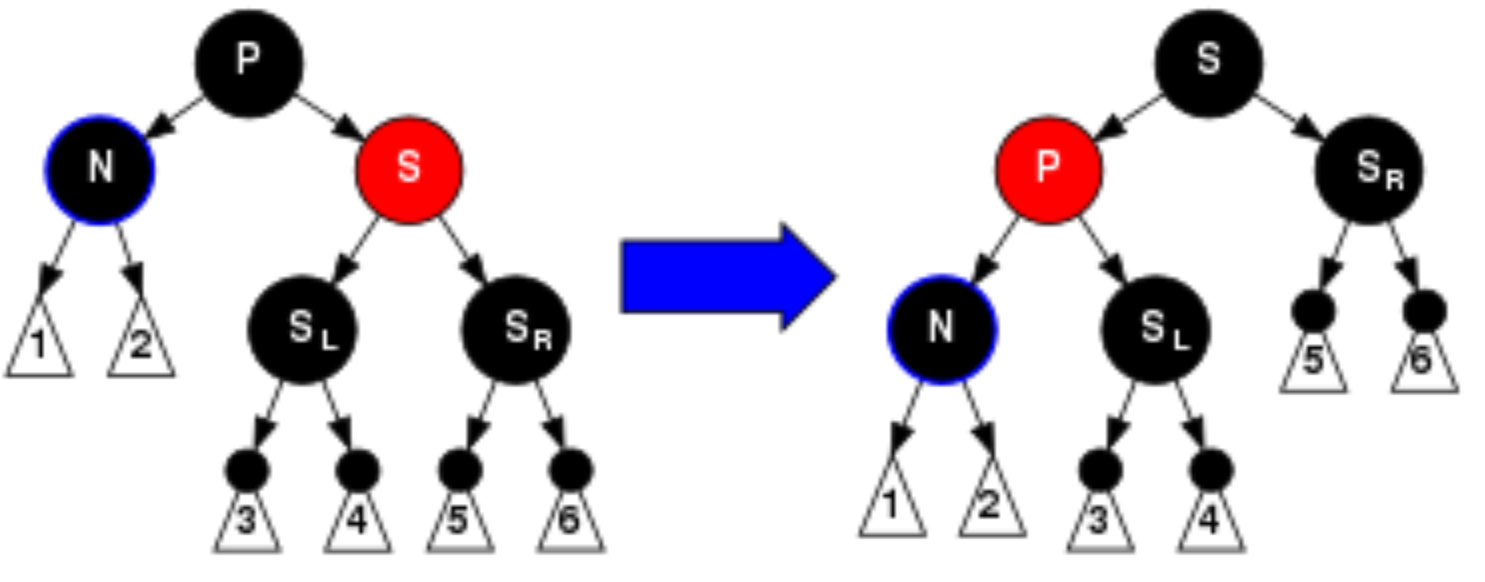
\includegraphics[width=0.5\textwidth]{redBlackRemoval1.png}
			\end{center}
		\end{itemize}
		Сильно лучше не стало, потому что поддеревья всё ещё имеют разную чёрную высоту, но теперь можно применить правила 4, 5 или 6
	\end{frame}

	\begin{frame}
		\frametitle{Красно-чёрные деревья, удаление}
		\framesubtitle{Случай 3}
		Если родитель чёрный, брат и его сыновья чёрные: перекрашиваем брата в красный. Поскольку из левого поддерева мы только что удалили один чёрный узел, а в правом поддереве один чёрный узел покрасили в красный, баланс восстановлен. Но только в поддереве, потому как оно стало на 1 чёрный узел короче, надо перебалансировать родителей.
		\begin{center}
			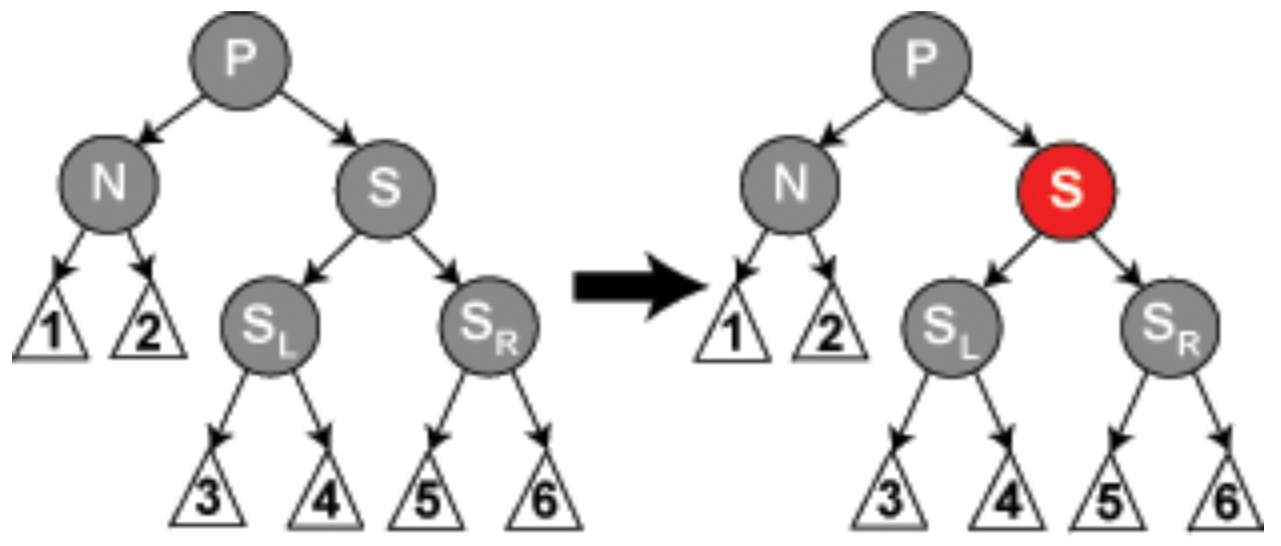
\includegraphics[width=0.5\textwidth]{redBlackRemoval2.png}
		\end{center}
	\end{frame}

	\begin{frame}
		\frametitle{Красно-чёрные деревья, удаление}
		\framesubtitle{Случай 4}
		Брат и сыновья брата чёрные, но родитель красный --- просто перекрасить брата нельзя. А вот перекрасить одновременно брата и родителя можно, это восстановит баланс (причём, во всём дереве сразу, потому что его чёрная высота не изменится).
		\begin{center}
			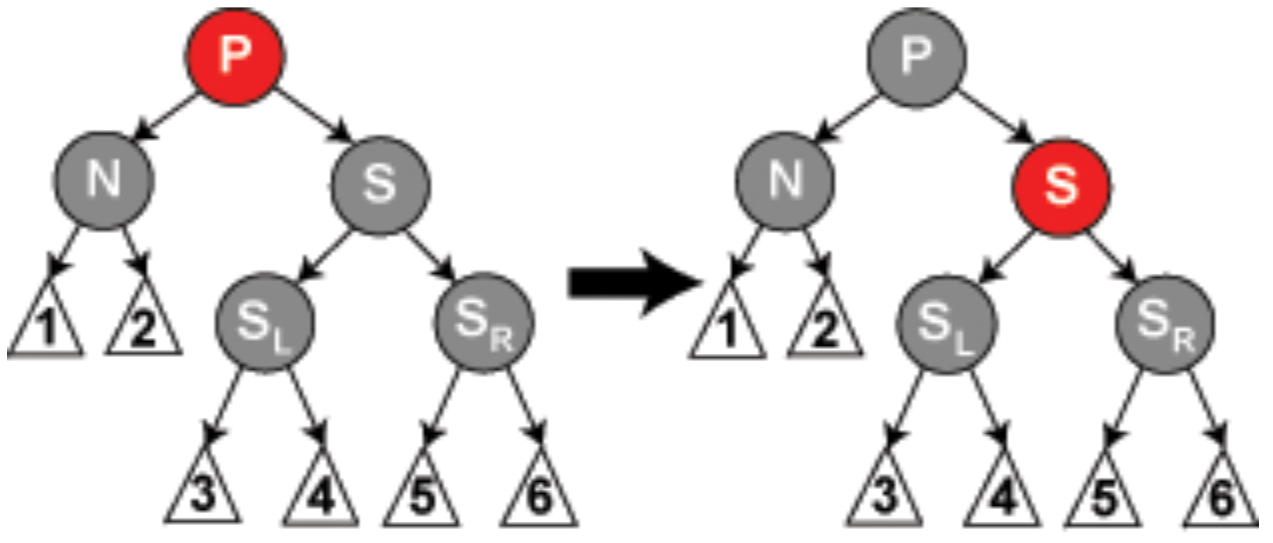
\includegraphics[width=0.5\textwidth]{redBlackRemoval3.png}
		\end{center}
	\end{frame}

	\begin{frame}
		\frametitle{Красно-чёрные деревья, удаление}
		\framesubtitle{Случай 5}
		Левый сын брата красный, правый --- чёрный. Выполняем поворот относительно брата и левого сына, одновременно перекрашивая брата и левого сына:
		\begin{center}
			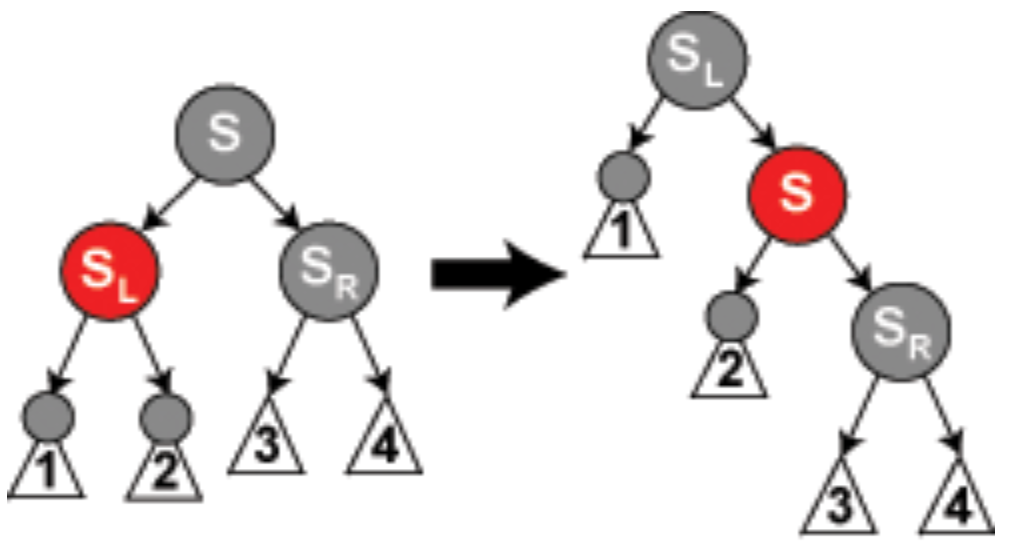
\includegraphics[width=0.4\textwidth]{redBlackRemoval4.png}
		\end{center}
		Глобально ничего не поменялось, но теперь можно применить случай 6.
	\end{frame}

	\begin{frame}
		\frametitle{Красно-чёрные деревья, удаление}
		\framesubtitle{Случай 6}
		Брат чёрный, его правый сын красный, левый --- чёрный: выполняем поворот вокруг ребра ``родитель-брат'' и перекрашиваем узлы:
		\begin{center}
			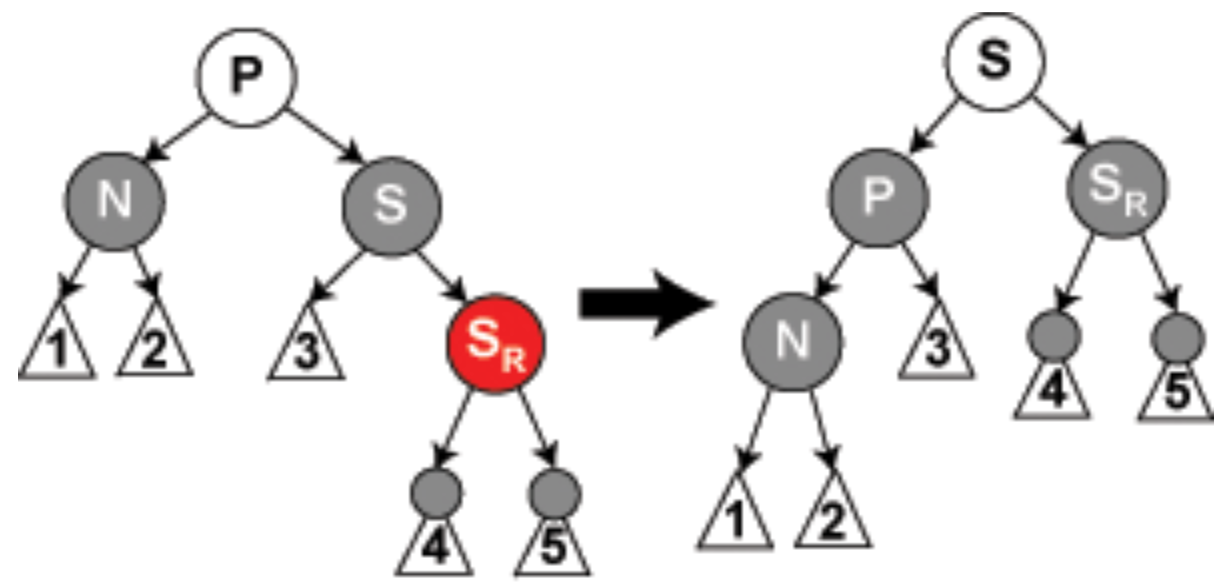
\includegraphics[width=0.5\textwidth]{redBlackRemoval5.png}
		\end{center}
		Баланс восстановлен (в левом поддереве на один чёрный узел больше), при этом можно доказать, что это всё ещё красно-чёрное дерево.
	\end{frame}

	\begin{frame}
		\frametitle{Splay-деревья}
		\begin{itemize}
			\item 1985г., Д. Слитор и Р.А. Тарьян
			\item Продвигает узлы, к которым часто происходит обращение, ближе к корню, поэтому может быть быстрее остальных деревьев
			\item Не хранит дополнительных данных в узлах
			\item Не гарантирует сбалансированности
			\item Не дружит с параллельными алгоритмами
			\item Проще в реализации
		\end{itemize}
	\end{frame}

	\begin{frame}
		\frametitle{Splay-деревья, splaying}
		Zig:\newline
		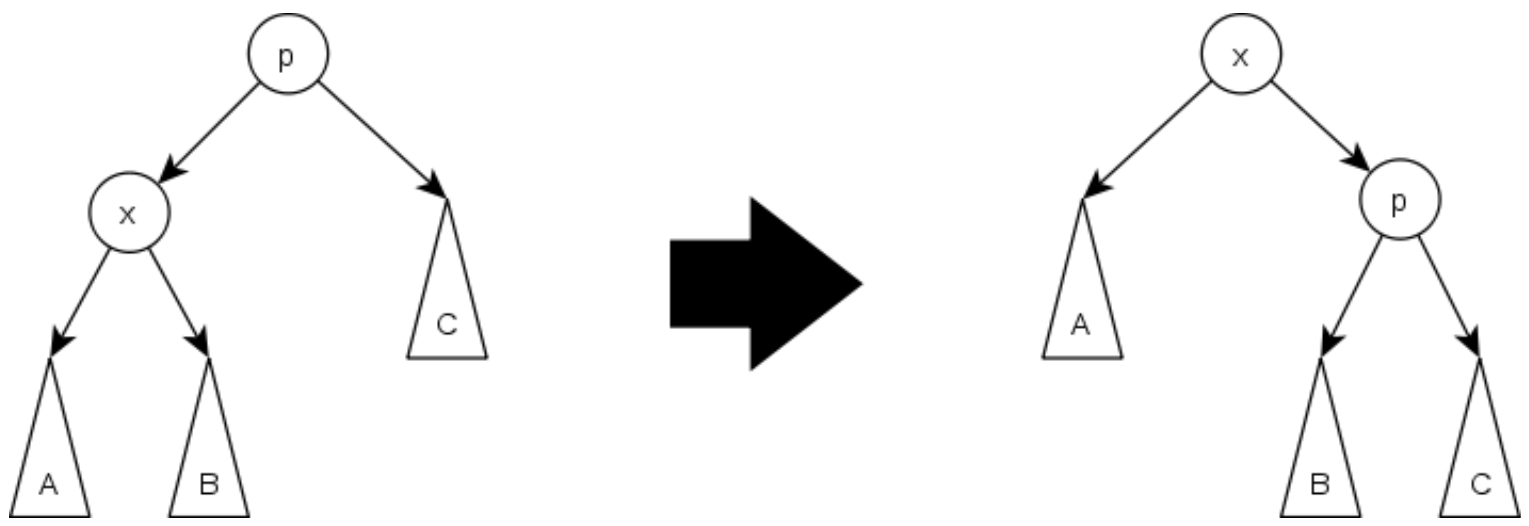
\includegraphics[width=0.4\textwidth]{splayZig.png}
		\vspace{5mm}
		\begin{columns}
			\begin{column}{0.5\textwidth}
				Zig-zag:\newline
				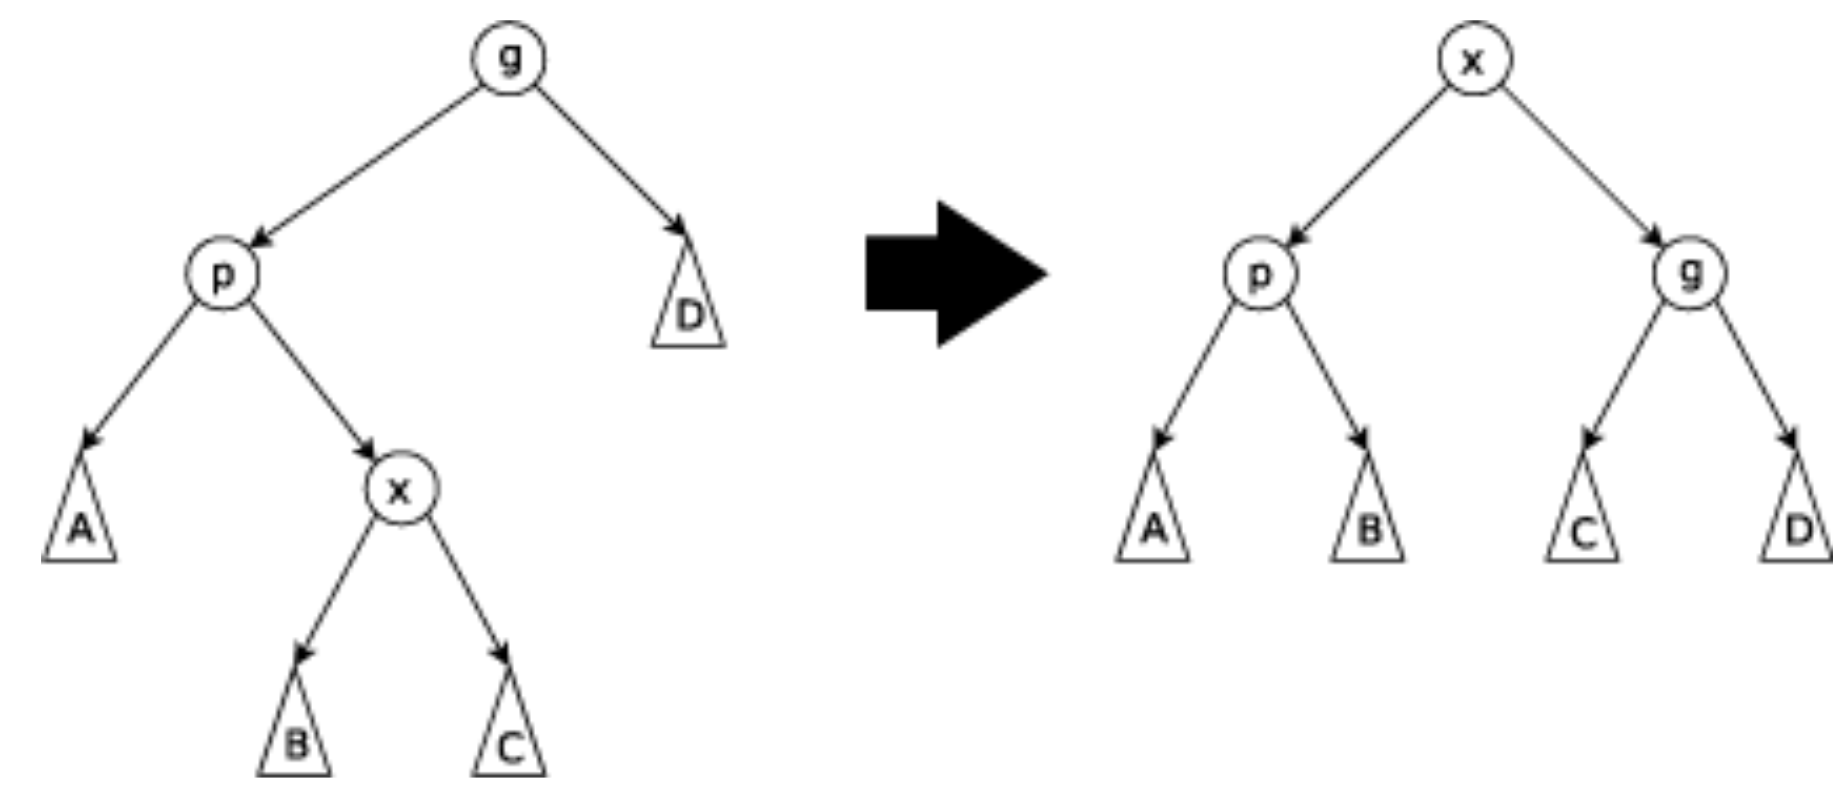
\includegraphics[width=0.9\textwidth]{splayZigZag.png}
			\end{column}
			\begin{column}{0.5\textwidth}
				Zig-zig:\newline
				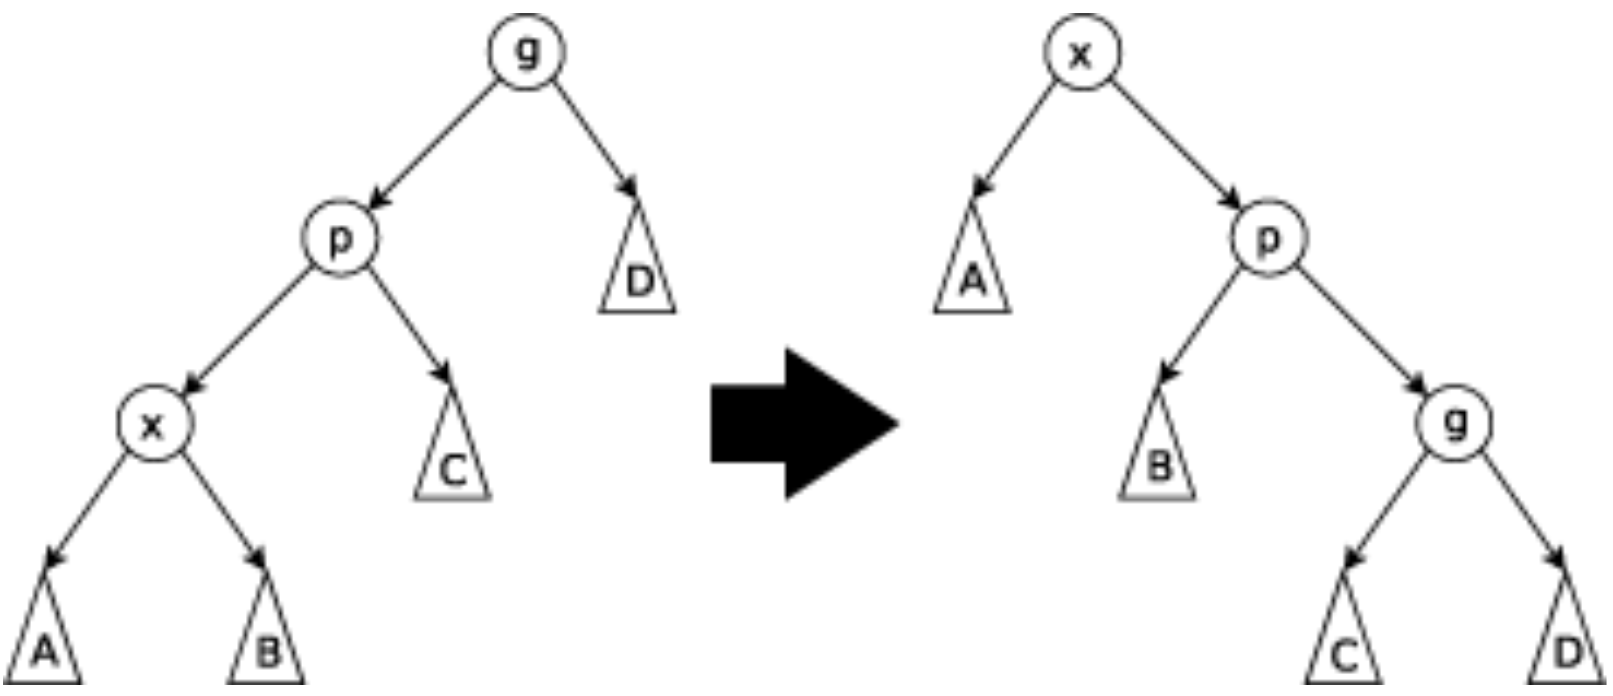
\includegraphics[width=0.9\textwidth]{splayZigZig.png}
			\end{column}
		\end{columns}
	\end{frame}

	\begin{frame}
		\frametitle{Splay-деревья, операции}
		\begin{itemize}
			\item Поиск:
			\begin{itemize}
				\item Ищем узел как в обычном двоичном дереве поиска
				\item Выполняем серию splaying-ов до тех пор, пока найденный узел не окажется корнем
			\end{itemize}
			\item Вставка:
			\begin{itemize}
				\item Вставляем узел как обычно в двоичное дерево поиска
				\item Выполняем серию splaying-ов до тех пор, пока вставленный узел не окажется корнем
			\end{itemize}
			\item Удаление:
			\begin{itemize}
				\item Удаляем узел как обычно
				\item Тащим родителя удалённого узла в корень дерева
			\end{itemize}
		\end{itemize}
	\end{frame}

	\begin{frame}
		\frametitle{Декартовы деревья}
		\begin{columns}
			\begin{column}{0.6\textwidth}
				\begin{itemize}
					\item Бинарное дерево поиска и куча одновременно
					\begin{itemize}
						\item Храним ключ и ``приоритет''
						\item Приоритет выбирается случайно (!) при добавлении ключа
						\item Куча по приоритету
					\end{itemize}
					\item Тоже лишь примерно сбалансировано
					\item Легко пишется
					\begin{itemize}
						\item Поэтому любимо олимпиадниками
					\end{itemize}
				\end{itemize}
			\end{column}
			\begin{column}{0.4\textwidth}
				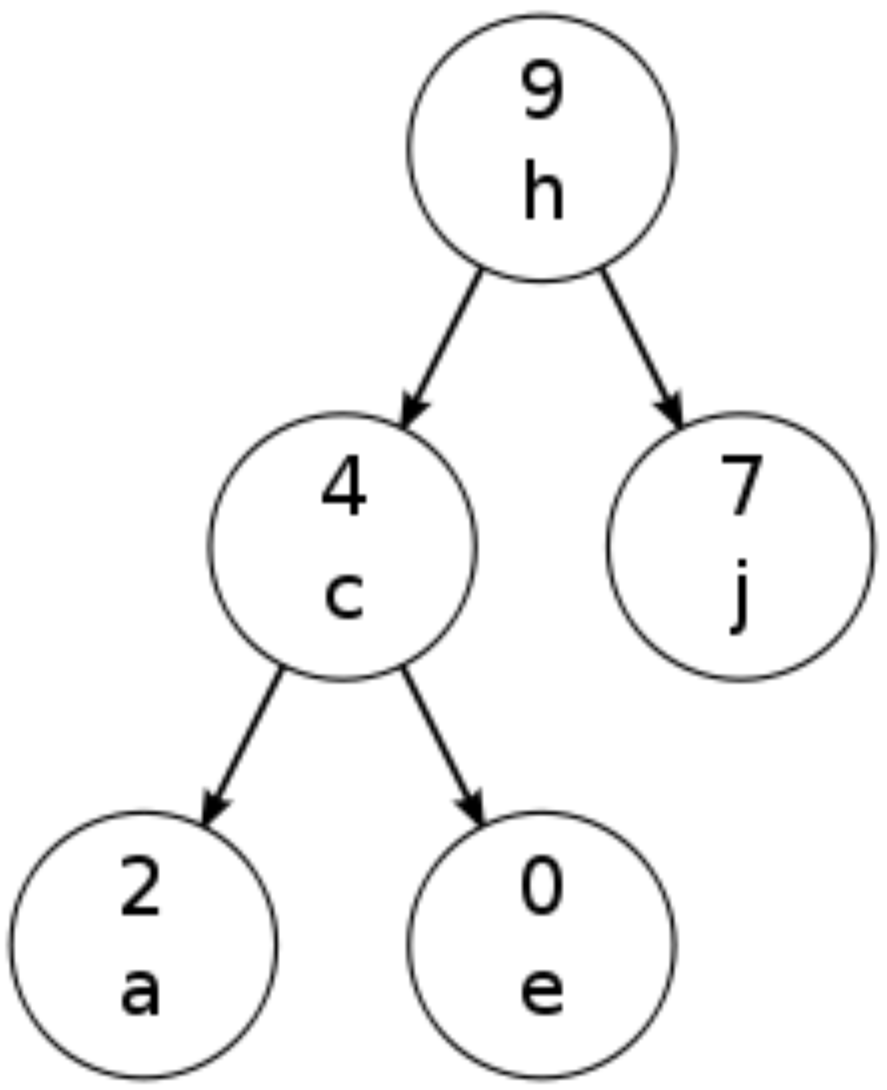
\includegraphics[width=0.7\textwidth]{treap.png}
			\end{column}
		\end{columns}
	\end{frame}

	\begin{frame}
		\frametitle{Декартово дерево и плоскость}
		\begin{center}
			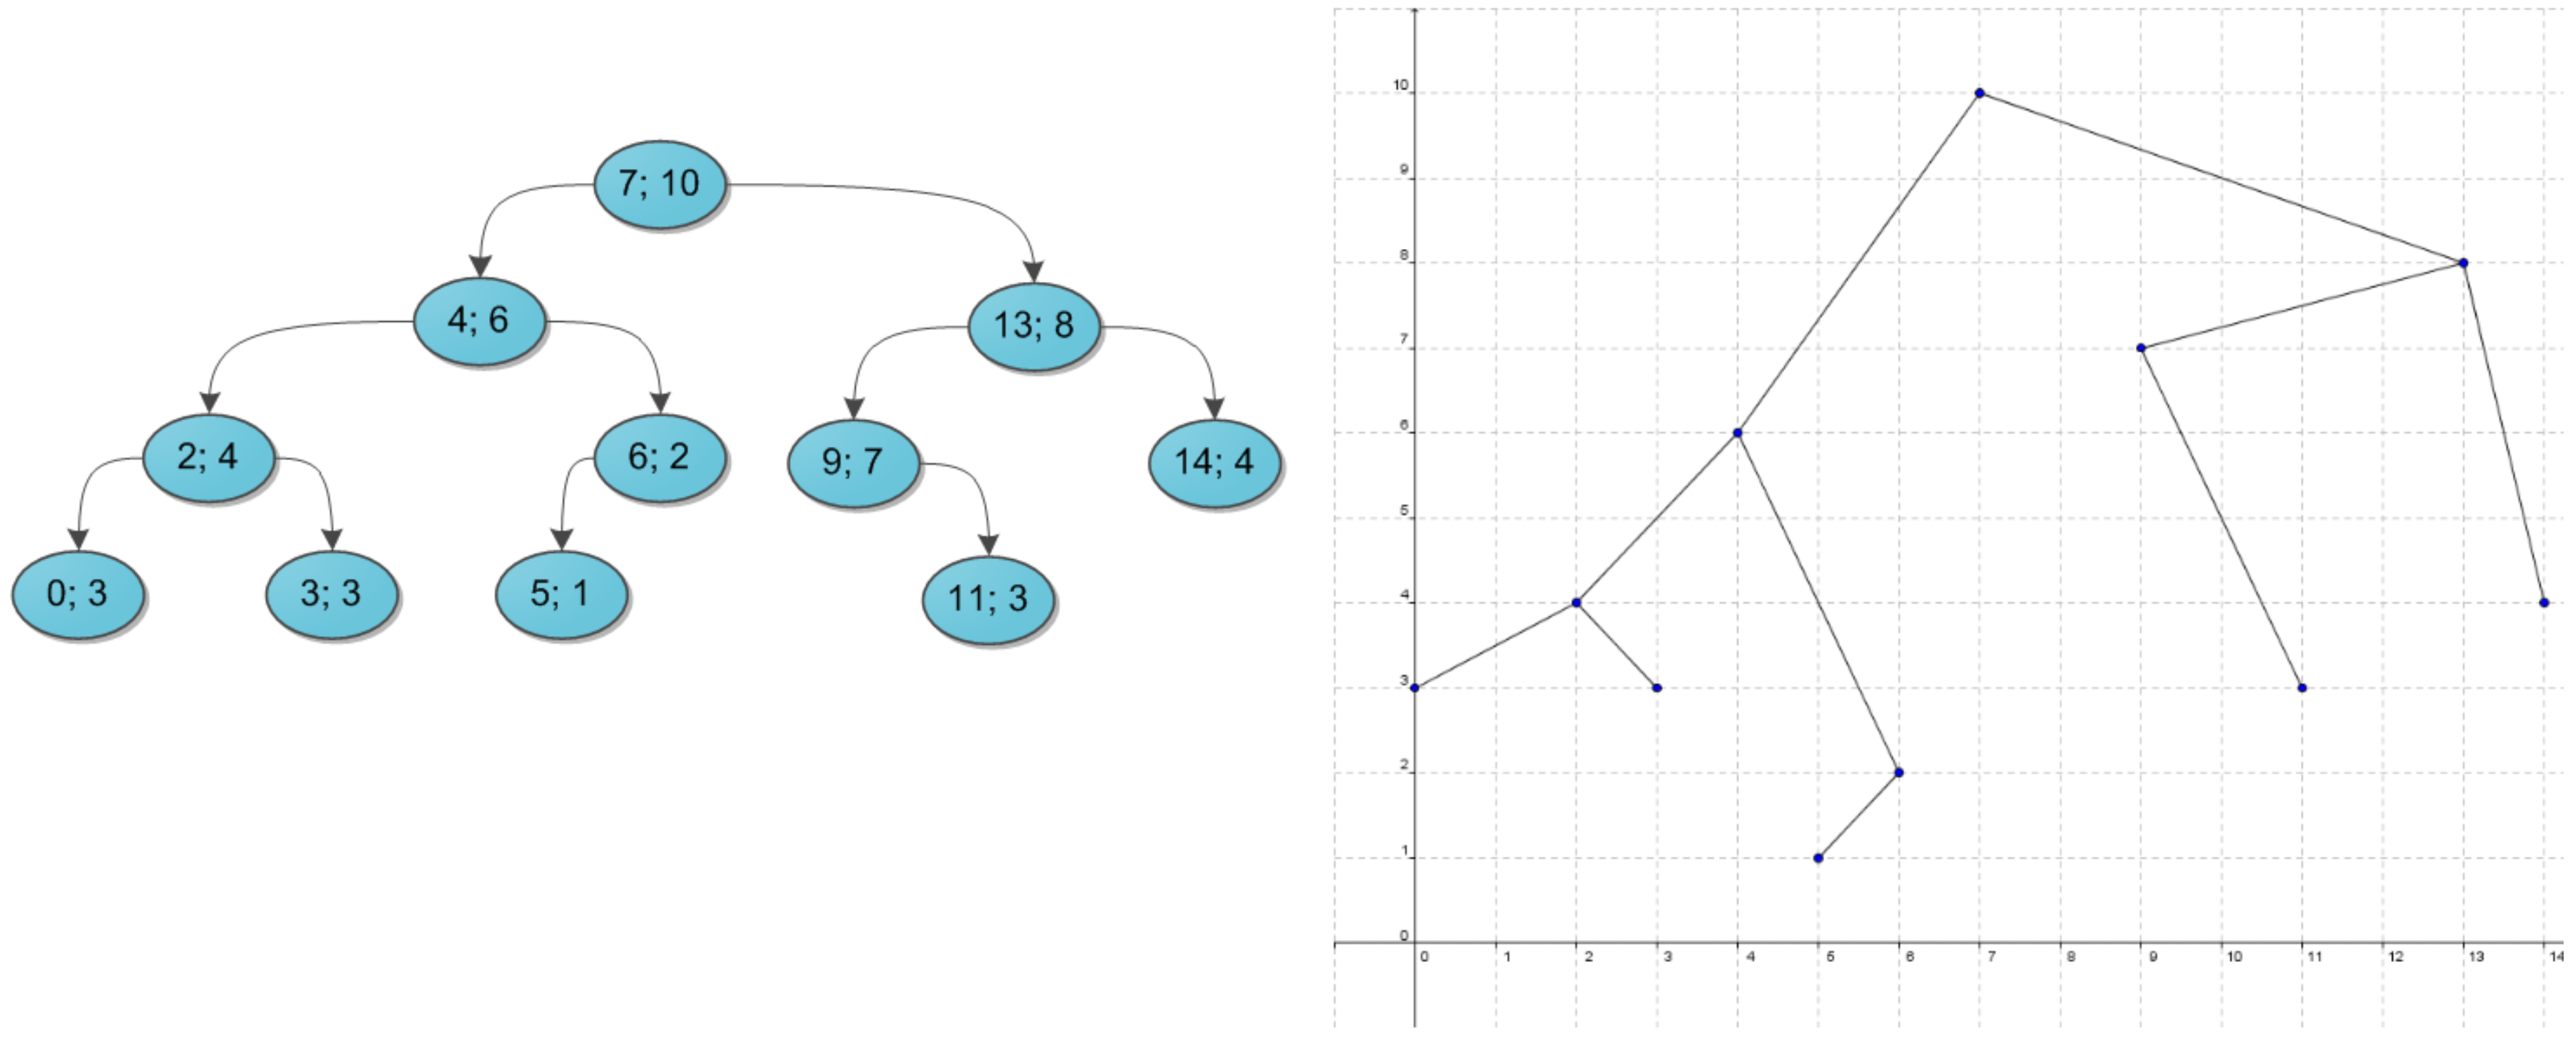
\includegraphics[width=\textwidth]{treapAndPlane.png}
		\end{center}
		\attribution{\url{https://habrahabr.ru/post/101818/}}
	\end{frame}

	\begin{frame}
		\frametitle{Merge}
		\begin{columns}
			\begin{column}{0.5\textwidth}
				\begin{itemize}
					\item Сливает два декартовых поддерева в одно
					\item Ключи в левом поддереве должны быть меньше ключей в правом
				\end{itemize}
			\end{column}
			\begin{column}{0.5\textwidth}
				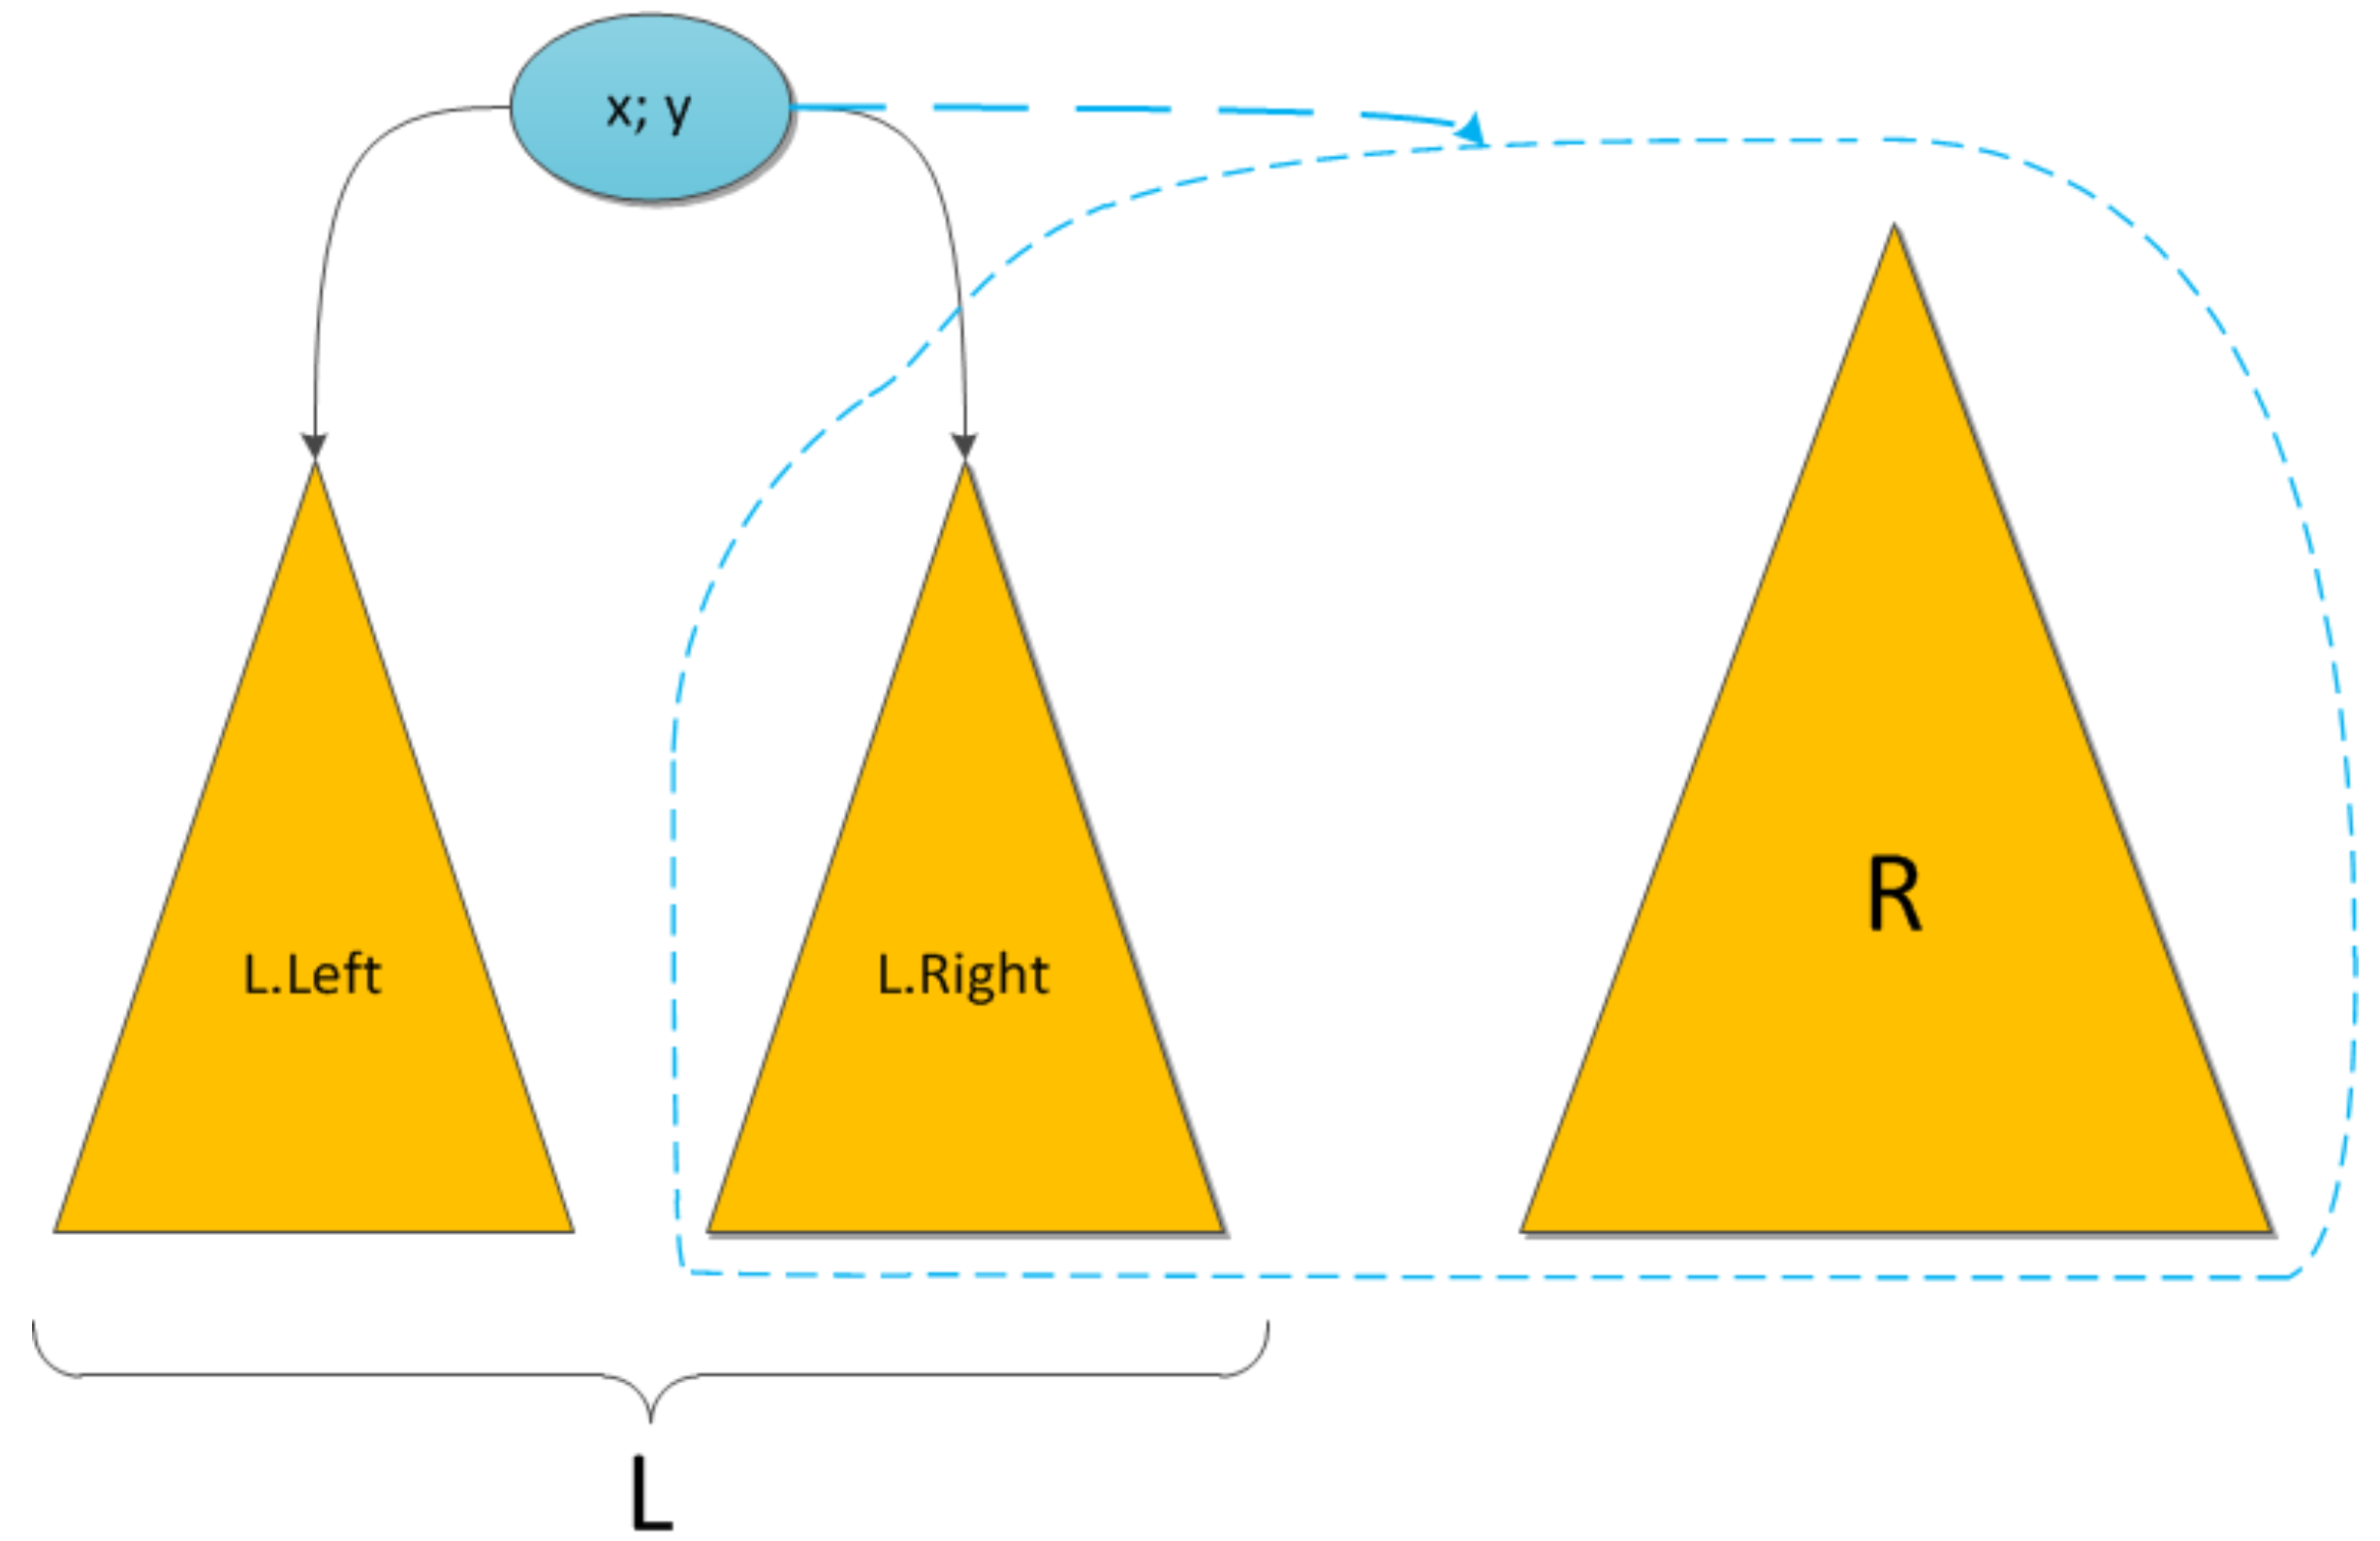
\includegraphics[width=0.9\textwidth]{treapMerge.png}
				\attribution{\url{https://habrahabr.ru/post/101818/}}
			\end{column}
		\end{columns}
	\end{frame}

	\begin{frame}
		\frametitle{Split}
		\begin{columns}
			\begin{column}{0.5\textwidth}
				\begin{itemize}
					\item Разделяет декартово дерево на два
					\item Ключи в левом меньше заданного, ключи в правом больше
				\end{itemize}
			\end{column}
			\begin{column}{0.5\textwidth}
				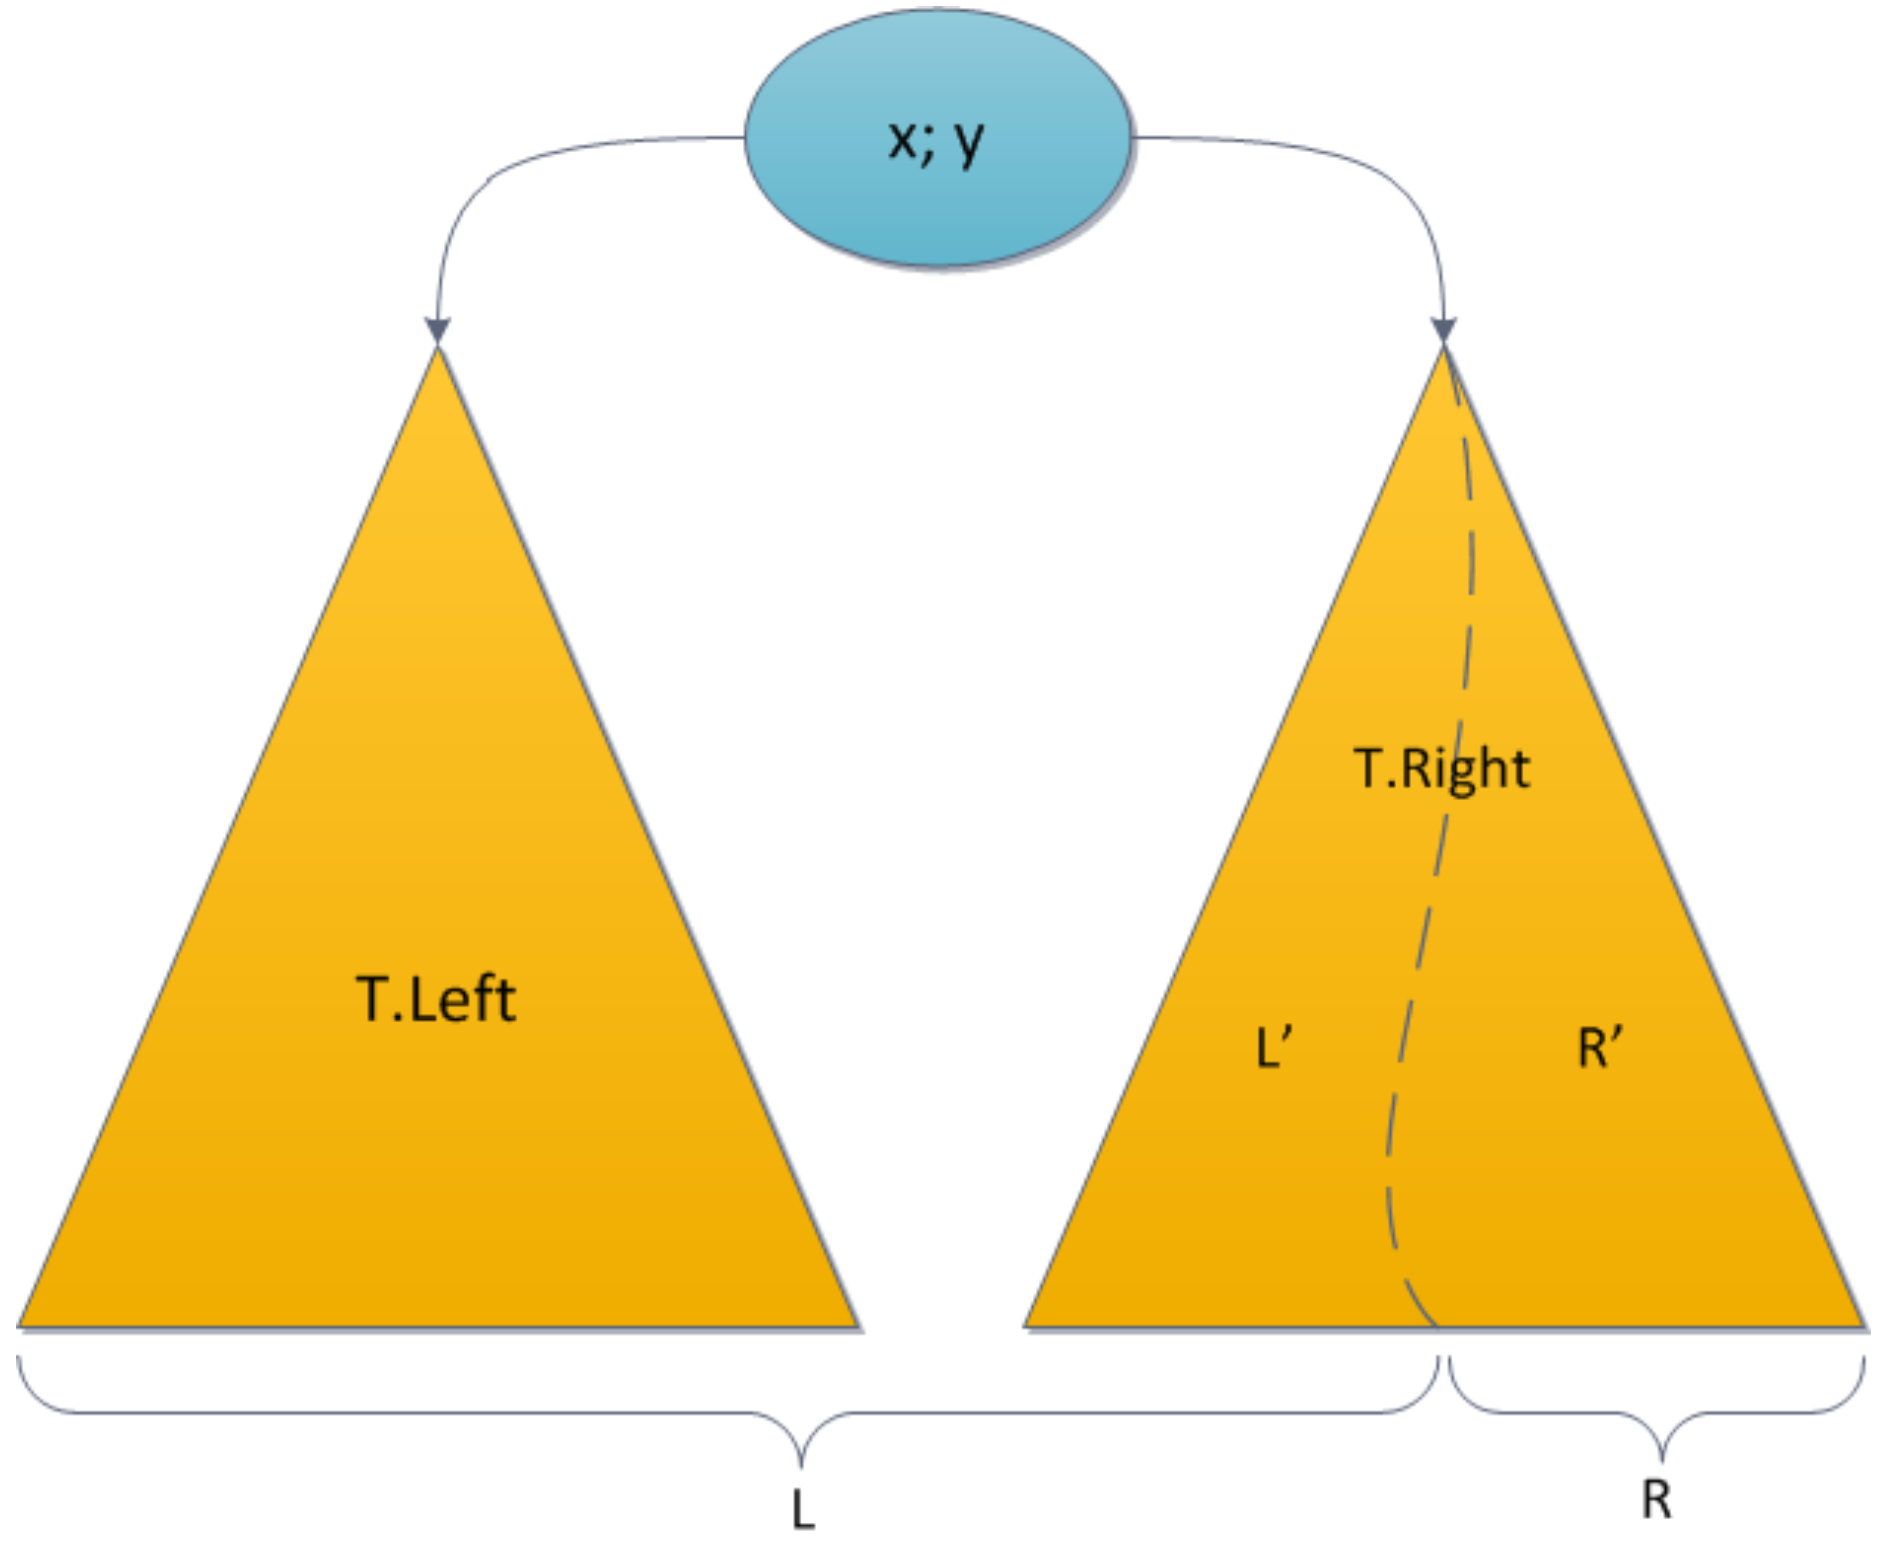
\includegraphics[width=0.9\textwidth]{treapSplit.png}
				\attribution{\url{https://habrahabr.ru/post/101818/}}
			\end{column}
		\end{columns}
	\end{frame}

	\begin{frame}
		\frametitle{Добавление}
		\begin{center}
			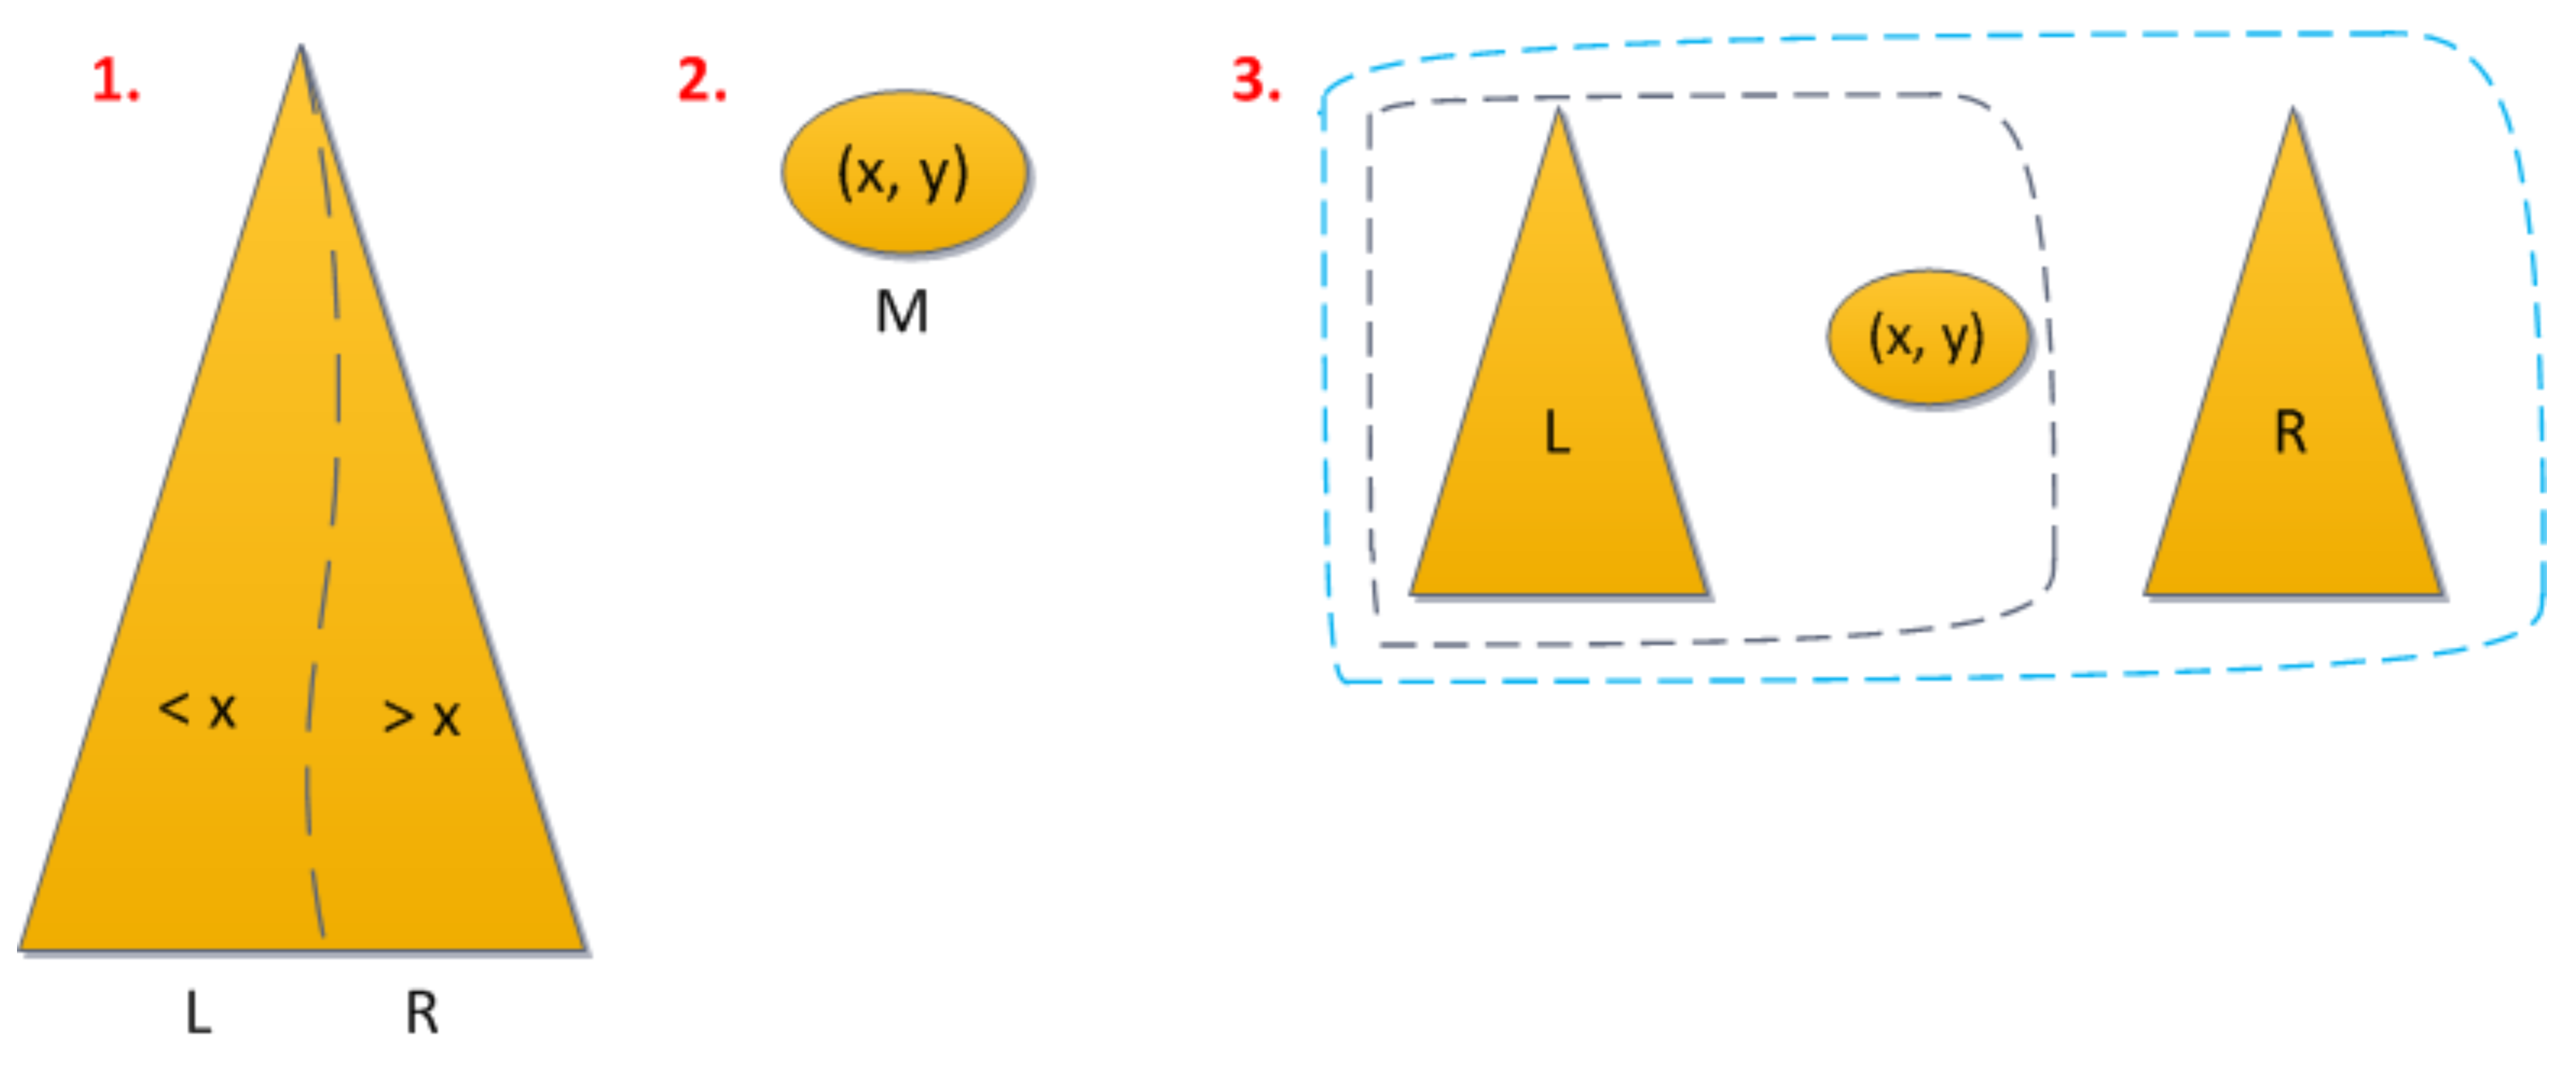
\includegraphics[width=\textwidth]{treapAddition.png}
		\end{center}
		\attribution{\url{https://habrahabr.ru/post/101818/}}
	\end{frame}

	\begin{frame}
		\frametitle{Удаление}
		\begin{center}
			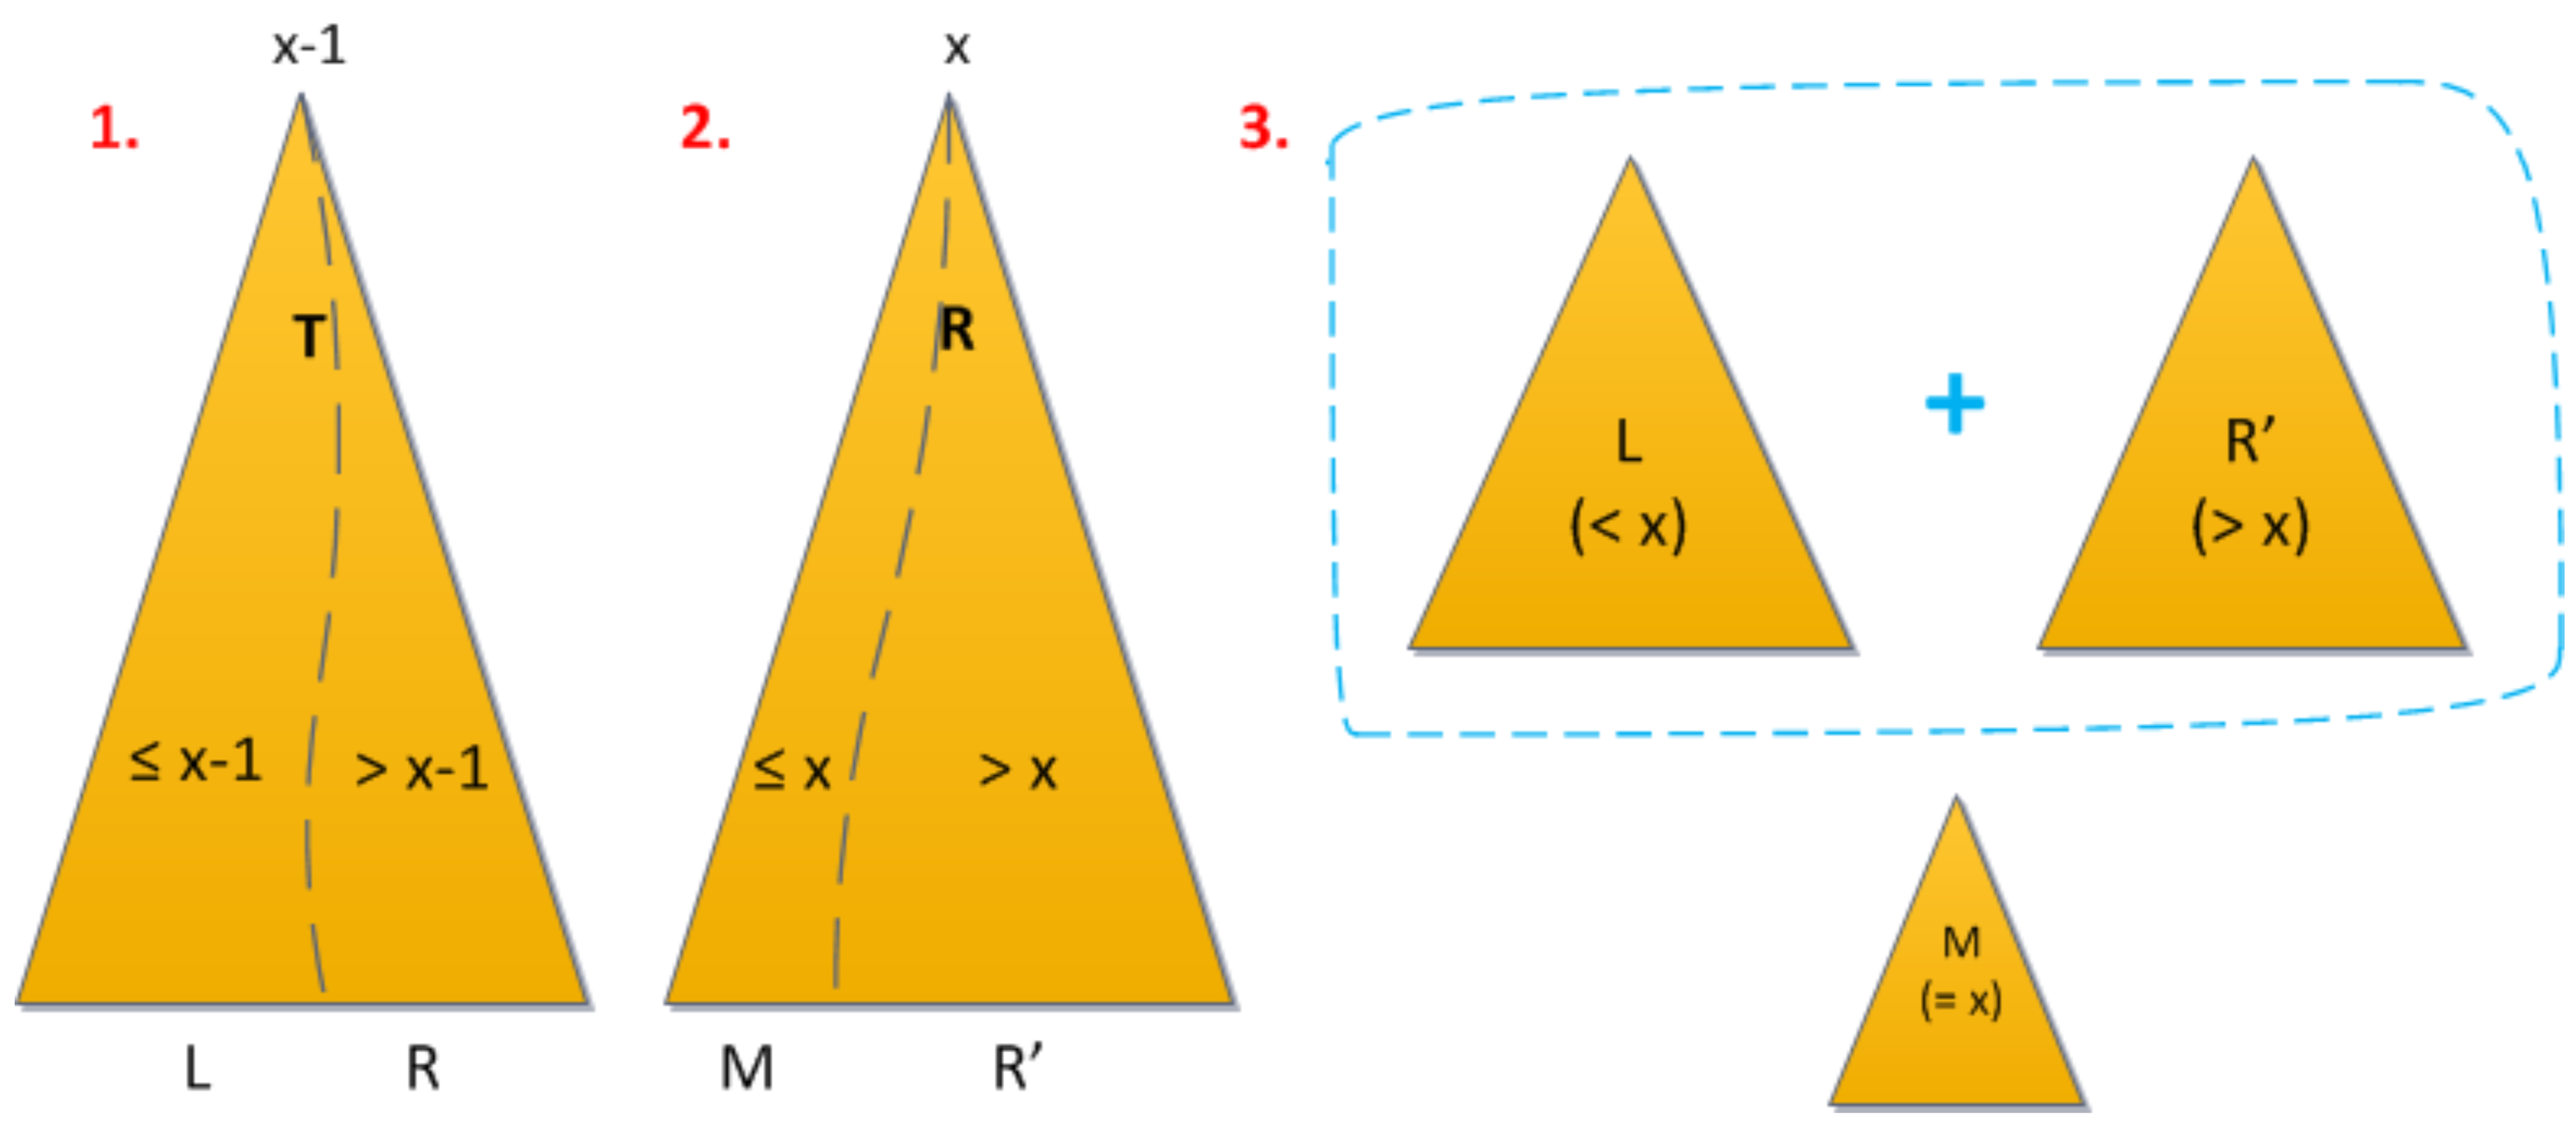
\includegraphics[width=\textwidth]{treapRemoval.png}
		\end{center}
		\attribution{\url{https://habrahabr.ru/post/101818/}}
	\end{frame}

	\section{Хеш-таблицы}

	\begin{frame}
		\frametitle{Хеш-таблицы}
		\begin{itemize}
			\item Реализация абстрактного типа данных ``множество'' или ``ассоциативный массив''
			\item Требует в среднем константного времени для операций вставки, удаления и поиска
			\begin{itemize}
				\item Очень похожа на массив
			\end{itemize}
			\item Хранит значения неупорядоченными
			\item Сильно зависит от качества хеш-функции
		\end{itemize}
	\end{frame}

	\begin{frame}
		\frametitle{Хеш-функция}
		\begin{columns}
			\begin{column}{0.6\textwidth}
				\begin{itemize}
					\item Некоторая функция, отображающая большое (потенциально бесконечное) множество \textbf{ключей} в конечное (и маленькое) множество \textbf{хеш-значений}
					\begin{itemize}
						\item Не инъективна
					\end{itemize}
					\item Чем ``случайнее'' она это делает, тем лучше
					\begin{itemize}
						\item Немного разным ключам должны соответствовать сильно разные значения
					\end{itemize}
				\end{itemize}
			\end{column}
			\begin{column}{0.4\textwidth}
				\begin{center}
					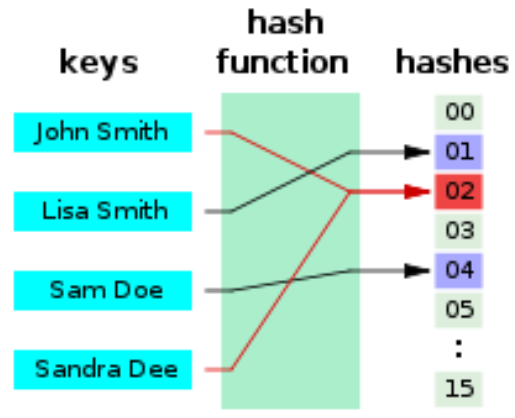
\includegraphics[width=0.8\textwidth]{hashFunction.png}
				\end{center}
			\end{column}
		\end{columns}
	\end{frame}

	\begin{frame}
		\frametitle{Хеш-функция}
		\begin{columns}
			\begin{column}{0.6\textwidth}
				\begin{itemize}
					\item Зачем
					\begin{itemize}
						\item Факторизуем множество ключей по классам эквивалентности, образованным ключами с равными хеш-значениями, будем хранить в массиве фактор-множества
						\item Хеш-значения можно использовать как индексы массива, где лежит что-то, что позволяет найти ключ (\textbf{сегменты}), и чем лучше хеш-функция перемешает ключи, тем меньше вероятность коллизии
					\end{itemize}
				\end{itemize}
			\end{column}
			\begin{column}{0.4\textwidth}
				\begin{center}
					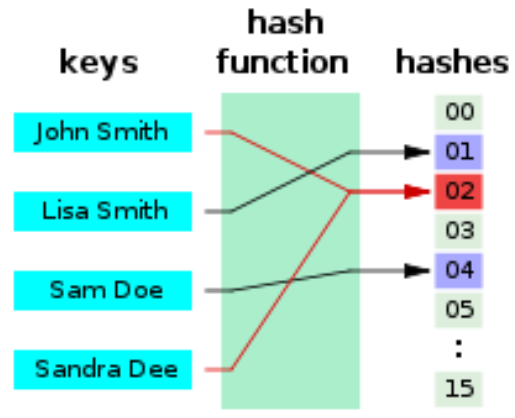
\includegraphics[width=0.8\textwidth]{hashFunction.png}
				\end{center}
			\end{column}
		\end{columns}
	\end{frame}

	\begin{frame}
		\frametitle{Хеш-таблица со списками значений}
		\begin{columns}
			\begin{column}{0.6\textwidth}
				\begin{itemize}
					\item Парадокс дней рождения: \\
					\textit{В группе, состоящей из 23 или более человек, вероятность совпадения дней рождения (число и месяц) хотя бы у двух людей превышает 50 \%}
					\item Будем хранить в массиве список ключей с одинаковым хеш-значением
				\end{itemize}
			\end{column}
			\begin{column}{0.4\textwidth}
				\begin{center}
					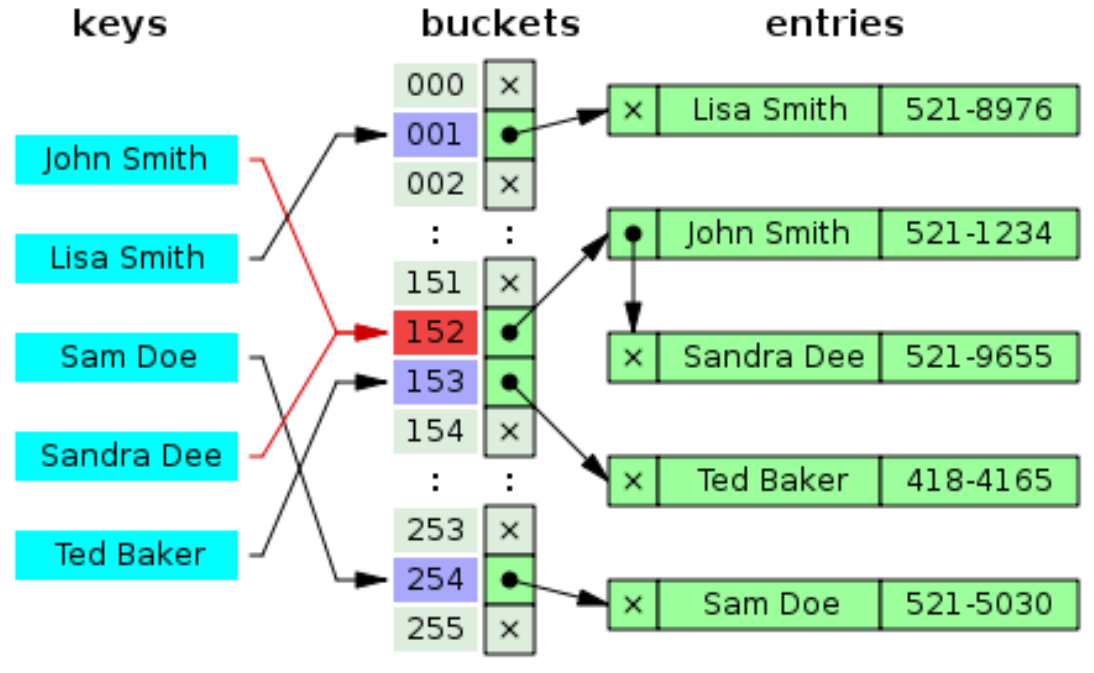
\includegraphics[width=\textwidth]{hashOnLists.png}
				\end{center}
			\end{column}
		\end{columns}
	\end{frame}

	\begin{frame}
		\frametitle{Хеш-таблица, ``открытая адресация''}
		\begin{columns}
			\begin{column}{0.6\textwidth}
				\begin{itemize}
					\item Второй способ: будем хранить в хеш-таблице сами ключи со значениями, а если ячейка уже занята, брать следующую (может быть, по какому-нибудь сложному правилу)
					\item Удаление требует дополнительной информации
					\begin{itemize}
						\item Пустая ячейка будет воспринята как конец цепочки
						\item Обычно делают флаг ``ячейка была удалена''
						\begin{itemize}
							\item При вставке --- вставляют
							\item При поиске и удалении --- идут дальше
						\end{itemize}
					\end{itemize}
				\end{itemize}
			\end{column}
			\begin{column}{0.4\textwidth}
				\begin{center}
					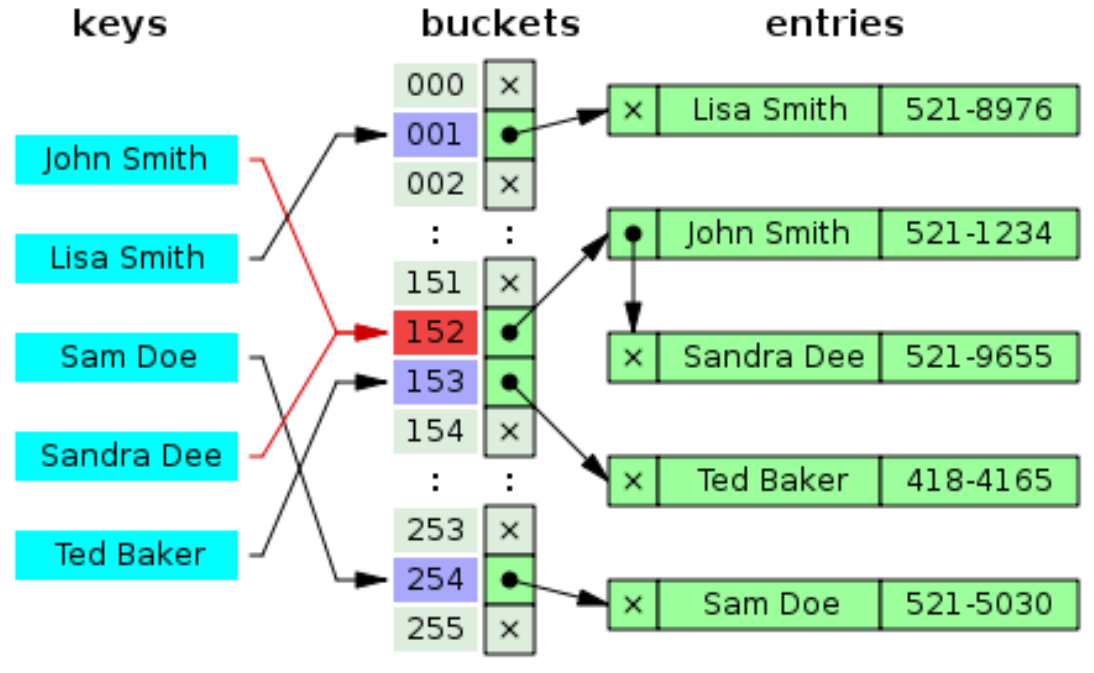
\includegraphics[width=\textwidth]{hashOnLists.png}
				\end{center}
			\end{column}
		\end{columns}
	\end{frame}

	\begin{frame}
		\frametitle{Коэффициент заполнения}
		\begin{itemize}
			\item Пусть $n$ --- число элементов в хеш-таблице, $k$ --- число сегментов (в английской литературе сегменты называются buckets). Коэффициент заполнения хеш-таблицы $L = n / k$
		\end{itemize}
		\begin{columns}
			\begin{column}{0.6\textwidth}
				\begin{itemize}
					\item Коэффициент заполнения должен быть примерно равен 1 для хеш-таблиц со списками и < 0.7 для хеш-таблиц с открытой адресацией
					\begin{itemize}
						\item Динамическое изменение размеров массива
					\end{itemize}
				\end{itemize}
			\end{column}
			\begin{column}{0.4\textwidth}
				\begin{center}
					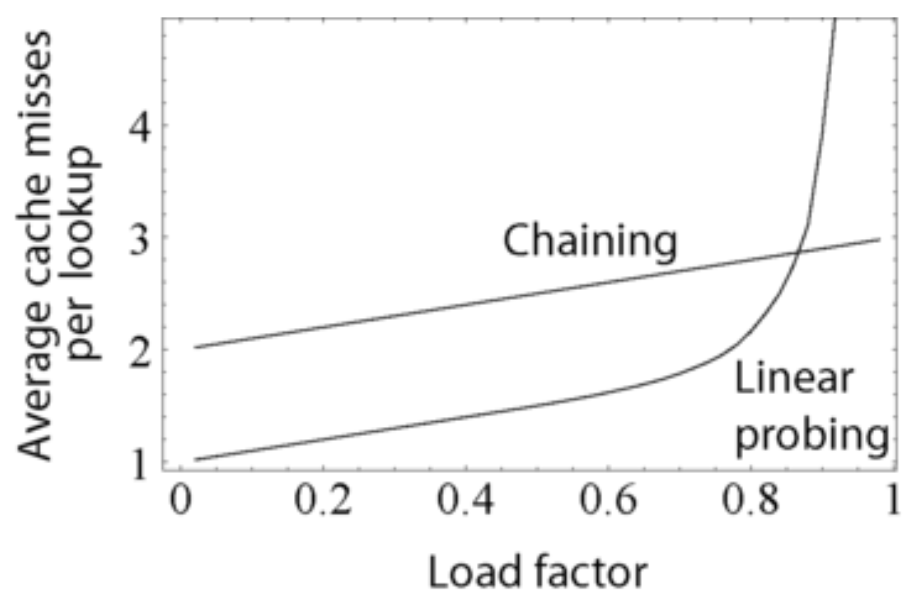
\includegraphics[width=\textwidth]{loadFactor.png}
				\end{center}
			\end{column}
		\end{columns}
	\end{frame}

	\begin{frame}[fragile]
		\frametitle{Выбор хеш-функции}
		\begin{itemize}
			\item Должна быть возможно более случайной
			\item Должна зависеть только от ключа
			\item Должна считаться быстро
			\item Например:
				\begin{minted}{c++}
int h(char *value) {
    int result = 0;
    for (int i = 0; value[i] != '\0'; ++i)
        result = (result + value[i]) % hashSize;
    return result;
}
				\end{minted}
			\item Обычно хеш-функция возвращает просто целое число, а хеш-таблица сама ``загоняет'' его в нужный диапазон значений
		\end{itemize}
	\end{frame}

	\begin{frame}
		\frametitle{Ещё про хеш-функции}
		\begin{itemize}
			\item Для целых чисел вполне сойдёт id
			\item ``Совершенная хеш-функция'' --- инъективна
			\item Универсальная хеш-функция --- семейство функций
			\item Криптографические хеш-функции
				\begin{itemize}
					\item MD5
					\item SHA1
					\item Небыстро считаются, поэтому не подходят
				\end{itemize}
			\item Хеш-функции для сложных типов данных
				\begin{itemize}
					\item Сумма или произведение хеш-функций элементов, как для строки
					\item Значение полинома $a[0]*p^n + a[1]*p^{n - 1} + … + a[n]$, особенно если $p$ --- простое
					\begin{itemize}
						\item Rolling hash
					\end{itemize}
					\item xor хеш-функций элементов
				\end{itemize}
		\end{itemize}
	\end{frame}

\end{document}